% Options for packages loaded elsewhere
\PassOptionsToPackage{unicode}{hyperref}
\PassOptionsToPackage{hyphens}{url}
%
\documentclass[
]{article}
\usepackage{amsmath,amssymb}
\usepackage{iftex}
\ifPDFTeX
  \usepackage[T1]{fontenc}
  \usepackage[utf8]{inputenc}
  \usepackage{textcomp} % provide euro and other symbols
\else % if luatex or xetex
  \usepackage{unicode-math} % this also loads fontspec
  \defaultfontfeatures{Scale=MatchLowercase}
  \defaultfontfeatures[\rmfamily]{Ligatures=TeX,Scale=1}
\fi
\usepackage{lmodern}
\ifPDFTeX\else
  % xetex/luatex font selection
\fi
% Use upquote if available, for straight quotes in verbatim environments
\IfFileExists{upquote.sty}{\usepackage{upquote}}{}
\IfFileExists{microtype.sty}{% use microtype if available
  \usepackage[]{microtype}
  \UseMicrotypeSet[protrusion]{basicmath} % disable protrusion for tt fonts
}{}
\makeatletter
\@ifundefined{KOMAClassName}{% if non-KOMA class
  \IfFileExists{parskip.sty}{%
    \usepackage{parskip}
  }{% else
    \setlength{\parindent}{0pt}
    \setlength{\parskip}{6pt plus 2pt minus 1pt}}
}{% if KOMA class
  \KOMAoptions{parskip=half}}
\makeatother
\usepackage{xcolor}
\usepackage[margin=1in]{geometry}
\usepackage{longtable,booktabs,array}
\usepackage{calc} % for calculating minipage widths
% Correct order of tables after \paragraph or \subparagraph
\usepackage{etoolbox}
\makeatletter
\patchcmd\longtable{\par}{\if@noskipsec\mbox{}\fi\par}{}{}
\makeatother
% Allow footnotes in longtable head/foot
\IfFileExists{footnotehyper.sty}{\usepackage{footnotehyper}}{\usepackage{footnote}}
\makesavenoteenv{longtable}
\usepackage{graphicx}
\makeatletter
\def\maxwidth{\ifdim\Gin@nat@width>\linewidth\linewidth\else\Gin@nat@width\fi}
\def\maxheight{\ifdim\Gin@nat@height>\textheight\textheight\else\Gin@nat@height\fi}
\makeatother
% Scale images if necessary, so that they will not overflow the page
% margins by default, and it is still possible to overwrite the defaults
% using explicit options in \includegraphics[width, height, ...]{}
\setkeys{Gin}{width=\maxwidth,height=\maxheight,keepaspectratio}
% Set default figure placement to htbp
\makeatletter
\def\fps@figure{htbp}
\makeatother
\setlength{\emergencystretch}{3em} % prevent overfull lines
\providecommand{\tightlist}{%
  \setlength{\itemsep}{0pt}\setlength{\parskip}{0pt}}
\setcounter{secnumdepth}{-\maxdimen} % remove section numbering
\ifLuaTeX
  \usepackage{selnolig}  % disable illegal ligatures
\fi
\IfFileExists{bookmark.sty}{\usepackage{bookmark}}{\usepackage{hyperref}}
\IfFileExists{xurl.sty}{\usepackage{xurl}}{} % add URL line breaks if available
\urlstyle{same}
\hypersetup{
  pdftitle={Funding Report: Goldberg Gator Engineering Explorers Summer Program 2023},
  pdfauthor={Krista D. Chisholm},
  hidelinks,
  pdfcreator={LaTeX via pandoc}}

\title{Funding Report: Goldberg Gator Engineering Explorers Summer
Program 2023}
\author{Krista D. Chisholm}
\date{2023-10-02}

\begin{document}
\maketitle

{
\setcounter{tocdepth}{2}
\tableofcontents
}
\hypertarget{summary}{%
\section{Summary}\label{summary}}

The Goldberg Gator Engineering Explorers (GGEE) Summer Program was
designed to provide middle school students with an authentic experience
in programming, engineering design, and computational thinking. The 2023
Summer Program successfully engaged 319 students across 8 school
districts. Students developed computational thinking skills through
design-based challenges using micro:bit micro-controllers.

Schools and Districts partnered with the GGEE program to host programs
and sponsor teachers and materials for the programs at their schools.
There were 20 local teachers that lead summer programs in their area.
Twenty undergraduate engineering students from the University of Florida
and neighboring colleges and universities supported teacher leaders and
served as mentors for students in the program. Both teachers and
undergraduate mentors were trained in program activities to upskill
their abilities in programming, computational thinking, engineering
desgin, and teaching practices. Two grant staff coordinated and ran the
programs.

----DATA

Demographics How students enjoyed the program Growth from beginning to
end

Follow up after-school programs in 5 districts for 12 sessions with
around 200 students participating in the program.

Program costs per student

\textbf{Last year summary} \emph{Students reported they felt challenged
during the program but were rewarded when their code or design worked.
They also mentioned the importance of collaboration with peers to solve
engineering problems, and they enjoyed the mentorship of the college
students working with the program. The longitudinal effects of the
summer program on grades in math and science and students' enrollment in
higher-level courses will be tracked by the research study for the
program. All districts provided in-kind donations to the camp, and many
school districts have plans to host or expand the programs for next
year. Some schools have asked about follow-up programming, including
afterschool programming to continue student engagement. The cost per
student for the program was \$996, including all costs for program
development (three months), camp costs (two months), and post-assessment
of the program. The cost per student for future camps should be less
owing to development costs built into the program's first year.}

\hypertarget{introduction}{%
\section{Introduction}\label{introduction}}

\hypertarget{background}{%
\subsection{Background}\label{background}}

The Goldberg Gator Engineering Explorers (GGEE) Summer Program was
initiated by a generous donor, Arnold Goldberg, to the University of
Florida Foundation. He envisioned a free summer program for
underrepresented minority middle school students. The program would
allow students and teachers to experience computer science and have
opportunities to learn to not only program but build skills in
computational thinking, problem solving, and engineering design. The
vision was brought to life by the Engaging Quality Instruction through
Professional Development (EQuIPD) grant at the University of Florida.
Their team worked with schools, districts, and teachers across Florida
to host these programs.

The GGEE Program was designed to introduce middle school-aged students
to programming and computer science. The program begins with students
learning the base elements of coding through small activities that
engage them in applying concepts such as strings, conditional
statements, loops, and variables. They use these concepts and the
micro:bit to develop a simple game and to also collect and analyze light
intensity data to study the relationship of light intensity and
distance. The program then has students working on two scaling design
challenges with partners and teams. The first is a creative engineering
design challenge where they create a micro:bit pet for a partner. Then
second is a technical design challenge where teams create a solution to
a local problem - traffic lights for emergency service vehicles,
environmental sensors for a farmer, and an indicator for new drivers.

An Advanced Program was developed and piloted during the second year of
the GGEE programs to allow returning students to continue to participate
in the GGEE programs. The program was designed to introduce students to
the basic concepts of Artificial Intelligence with a focus in Machine
Learning. The Advanced Program session designed to be held over 4
full-days. Registrations were open to students who previously attended
the GGEE program in 2022.

\hypertarget{purpose-of-the-report}{%
\subsection{Purpose of the Report}\label{purpose-of-the-report}}

This funding report provides an overview of the 2023 Goldberg Gator
Engineering Explorer Summer Programs. The report provides details from
preparing for the summer programs, during the summer program, and
information about what follows the programs as well as suggestions for
next year's programs.

\hypertarget{preparation-for-ggee-programs}{%
\section{Preparation for GGEE
Programs}\label{preparation-for-ggee-programs}}

To prepare for the GGEE Summer Programs, the EQuIPD team worked to
recruit school districts, students, and prepare required research
documentation.

\hypertarget{school-district-recruitment}{%
\subsection{School District
Recruitment}\label{school-district-recruitment}}

\emph{Detail the strategies used to recruit students for the program.
Discuss any partnerships or collaborations that helped with recruitment
efforts.}

\textbf{October 2022}

Emails were sent to schools and districts to invite them to participate
in the 2023 Goldberg Gator Engineering Explorer Programs. Correspondence
was sent to schools that participated in the 2022 pilot programs in
addition to all of the school district leaders in Career and Technical
Education across Florida. The email provided an overview of the program
and it's pilot run in 2022. It also contained a survey for schools or
districts to sign up to show their interest and to learn more about the
program in an upcoming information session. These emails were
distributed multiple times up until the information session.

The information session was held on October, 13th, 2022 and had 11
registrants from Broward, Hillsborough, Lake, Manatee, Miami-Dade, Palm
Beach, Santa Rosa, and St.~Lucie counties.

\begin{itemize}
\tightlist
\item
  working with schools and districts to coordinate programs and funding
\end{itemize}

\textbf{November 2022}

School recruitment for the 2023 GGEE Summer Programs began in November
of 2022. Flyers were shared via email to school administration

\begin{longtable}[]{@{}ll@{}}
\caption{2023 Goldberg Gator Engineering Summer Program location funding
sources.}\tabularnewline
\toprule\noalign{}
School District & Program Funding \\
\midrule\noalign{}
\endfirsthead
\toprule\noalign{}
School District & Program Funding \\
\midrule\noalign{}
\endhead
\bottomrule\noalign{}
\endlastfoot
Alachua County Schools & Local Funding \\
Brevard Public Schools & UF Donor Funding \\
City of Rivieria Beach - Palm Beach County & City Funded \\
Miami Dade County Public Schools & UF - GGEE Donor Funding \\
Orange County Public Schools & District Funding \\
Pinellas County Schools & District Funding \\
Santa Rosa County District Schools & District Funding \\
Sarasota County Schools & District Funding \\
School District of Palm Beach County & District Funding \\
\end{longtable}

\hypertarget{student-recruitment}{%
\subsection{Student Recruitment}\label{student-recruitment}}

\emph{Explain the criteria used to select participants for the program.
This could include grade level, academic standing, or other factors.}

School Recruitment

\hypertarget{research-and-youth-compliance}{%
\subsection{Research and Youth
Compliance}\label{research-and-youth-compliance}}

\hypertarget{research}{%
\subsubsection{Research}\label{research}}

\begin{itemize}
\tightlist
\item
  IRB filed through UF for research
\item
  Research questions
\item
  Surveys
\item
  Interview Protocols
\item
  Parent Research Consent
\end{itemize}

\hypertarget{youth-compliance}{%
\subsubsection{Youth Compliance}\label{youth-compliance}}

\begin{itemize}
\tightlist
\item
  Mentors Level 2 Background Screening and Fingerprinting for Jessica
  Lundsford Act
\item
  School district partnership covered compliance for their teachers
\item
  UF Youth Compliance Training
\item
  UF Waiver liability\ldots\ldots for Parents
\end{itemize}

\hypertarget{scheduling-summer-programs}{%
\section{Scheduling Summer Programs}\label{scheduling-summer-programs}}

\hypertarget{vs.-2023}{%
\subsection{2022 vs.~2023}\label{vs.-2023}}

The program was piloted during the Summer of 2022 with eight sessions
and six school districts. The program served just over 100 hundred
students. The pilot summer program paved the way for a pilot year of
virtual after-school programs during the 2022-2023 school year. Student
joined the sessions remotely from home. The 2023 summer program
\#\#\#\#\#\#\#\#\#\#\#\#\#\#\#\#\#\#\#\#\#\#\#\#\#\#\#\#\#\#\#\#\#

\begin{figure}
\centering
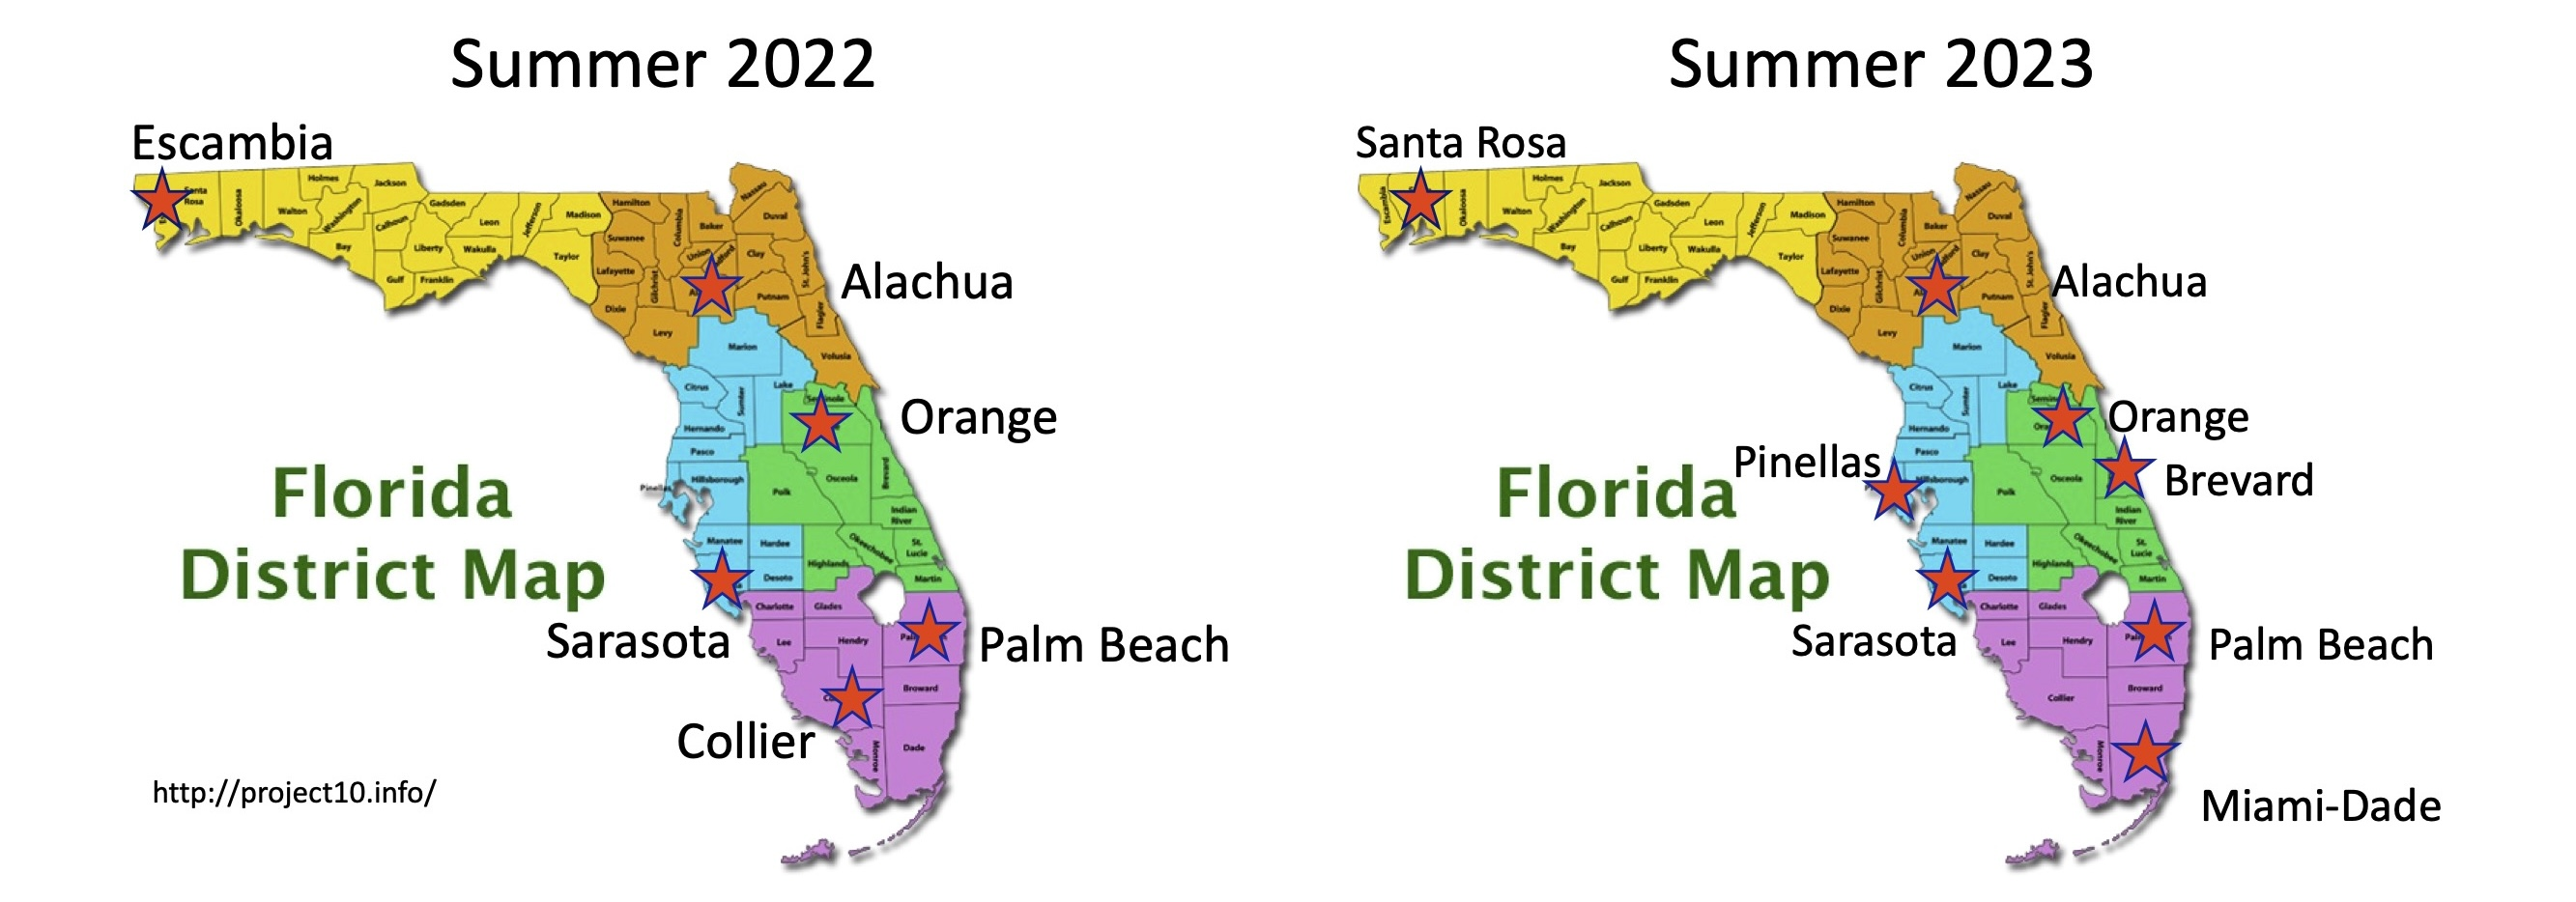
\includegraphics{Images/GGEE_23_FL District Map.jpg}
\caption{\emph{GGEE Summer Program Districts from 2022 and 2023}}
\end{figure}

\begin{longtable}[]{@{}llll@{}}
\caption{2023 Goldberg Gator Engineering Summer Program Locations,
Programs, and Formats.}\tabularnewline
\toprule\noalign{}
School District & School/Organization Name & Program Level & Format \\
\midrule\noalign{}
\endfirsthead
\toprule\noalign{}
School District & School/Organization Name & Program Level & Format \\
\midrule\noalign{}
\endhead
\bottomrule\noalign{}
\endlastfoot
Alachua County Schools & Take Stock In Children & Advanced & 2-day,
Full \\
Brevard Public Schools & Stone Middle School & Introductory & 4-day,
Full \\
City of Rivieria Beach - Palm Beach County & Youth Empowerment Programs
& Introductory & 8-day, Half \\
Miami Dade County Public Schools & Homestead Senior High School &
Introductory & 8-day, Half \\
Miami Dade County Public Schools & North Miami Beach Senior High &
Introductory & 8-day, Half \\
Orange County Public Schools & University High School & Introductory &
4-day, Full \\
Orange County Public Schools & University High School & Advanced &
4-day, Full \\
Orange County Public Schools & University High School & Introductory &
4-day, Full \\
Orange County Public Schools & University High School & Introductory &
4-day, Full \\
Pinellas County Schools & East Lake High School & Introductory & 4-day,
Full \\
Pinellas County Schools & Lakewood High School & Introductory & 4-day,
Full \\
Santa Rosa County District Schools & Central School & Introductory &
8-day, Half \\
Santa Rosa County District Schools & Gulf Breeze High School &
Introductory & 8-day, Half \\
Santa Rosa County District Schools & Gulf Breeze High School &
Introductory & 8-day, Half \\
Santa Rosa County District Schools & Milton High School & Introductory &
8-day, Half \\
Santa Rosa County District Schools & Navarre High School & Introductory
& 8-day, Half \\
Santa Rosa County District Schools & Navarre High School & Introductory
& 8-day, Half \\
Sarasota County Schools & Booker Middle School & Introductory & 4-day,
Full \\
Sarasota County Schools & Booker Middle School & Advanced & 4-day,
Full \\
School District of Palm Beach County & Bear Lakes Middle School &
Introductory & 8-day, Half \\
School District of Palm Beach County & Carver Middle School &
Introductory & 8-day, Half \\
School District of Palm Beach County & Lake Shore Middle School &
Introductory & 8-day, Half \\
\end{longtable}

\hypertarget{program-calendar}{%
\subsection{Program Calendar}\label{program-calendar}}

\emph{Provide an overview of the program's calendar, including the
duration of the program, daily schedules, and key activities.}

There were X many programs in each district

\begin{figure}
\centering
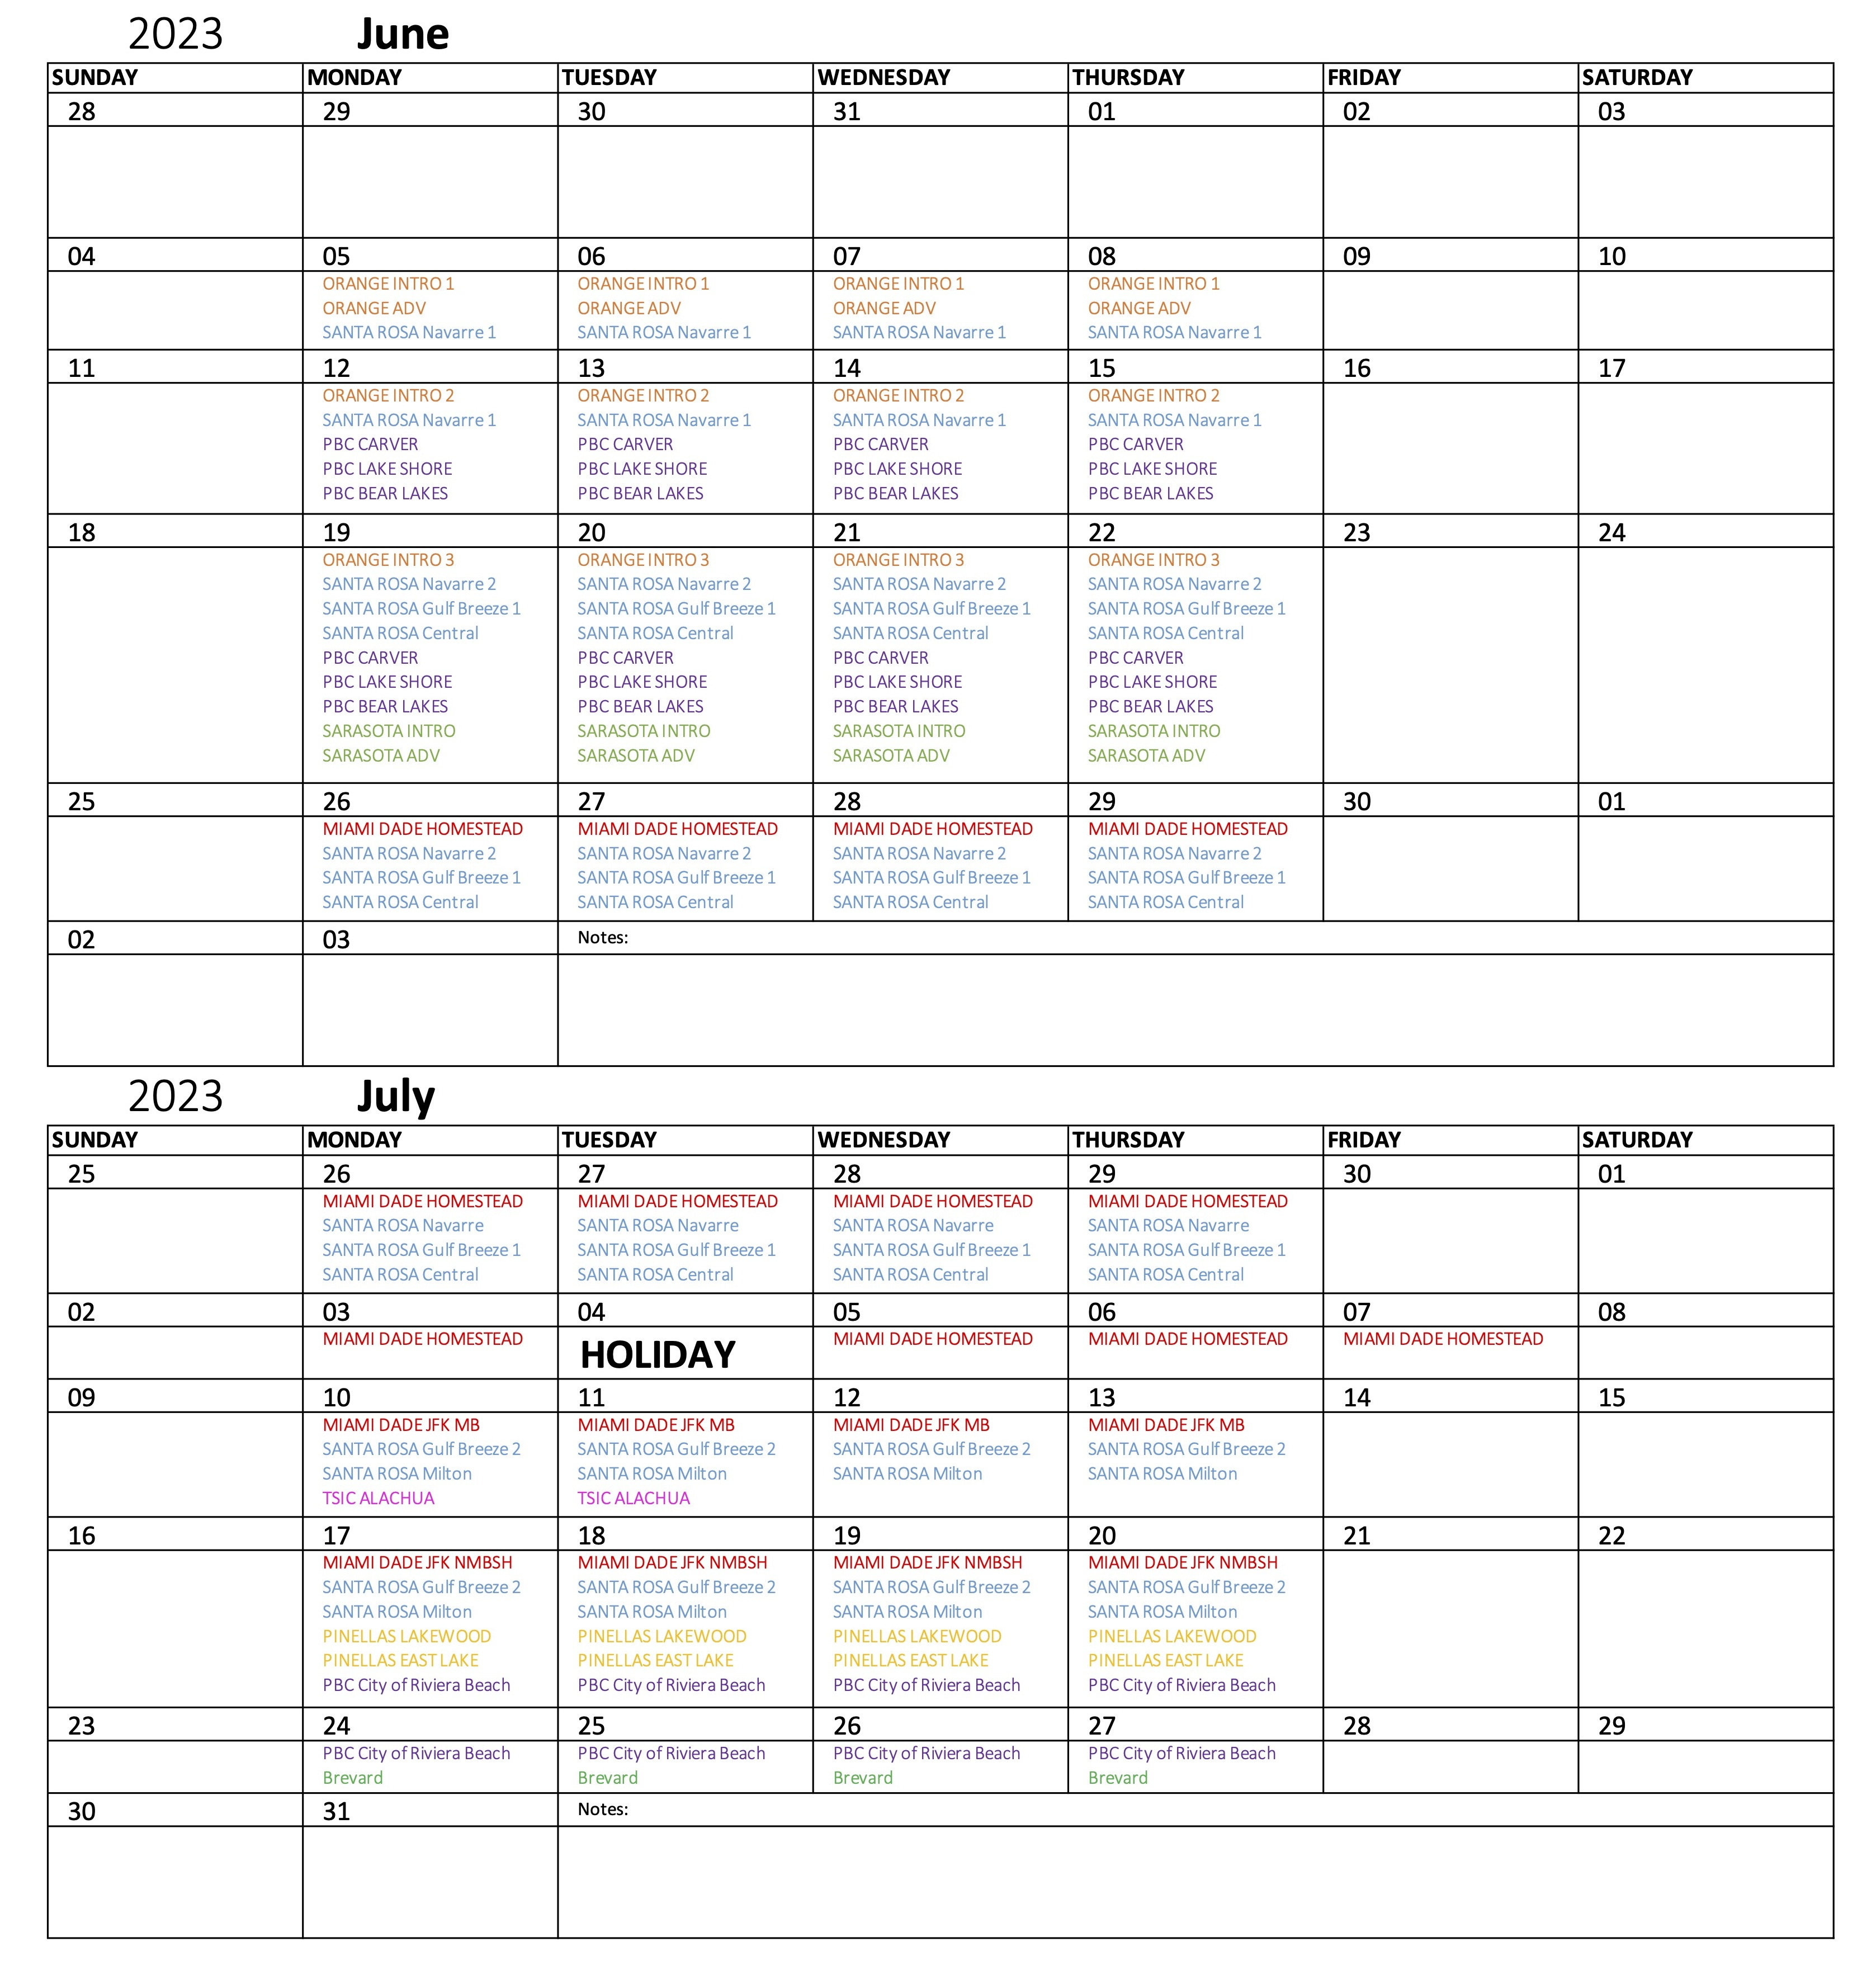
\includegraphics[width=1\textwidth,height=\textheight]{Images/GGEE_23_Calendar.jpg}
\caption{\emph{2023 Goldberg Gator Engineering Explorers Summer Program
Calendar}}
\end{figure}

\hypertarget{program-layouts}{%
\section{Program Layouts}\label{program-layouts}}

\hypertarget{introductory-programs}{%
\subsection{Introductory Programs}\label{introductory-programs}}

\begin{figure}
\centering
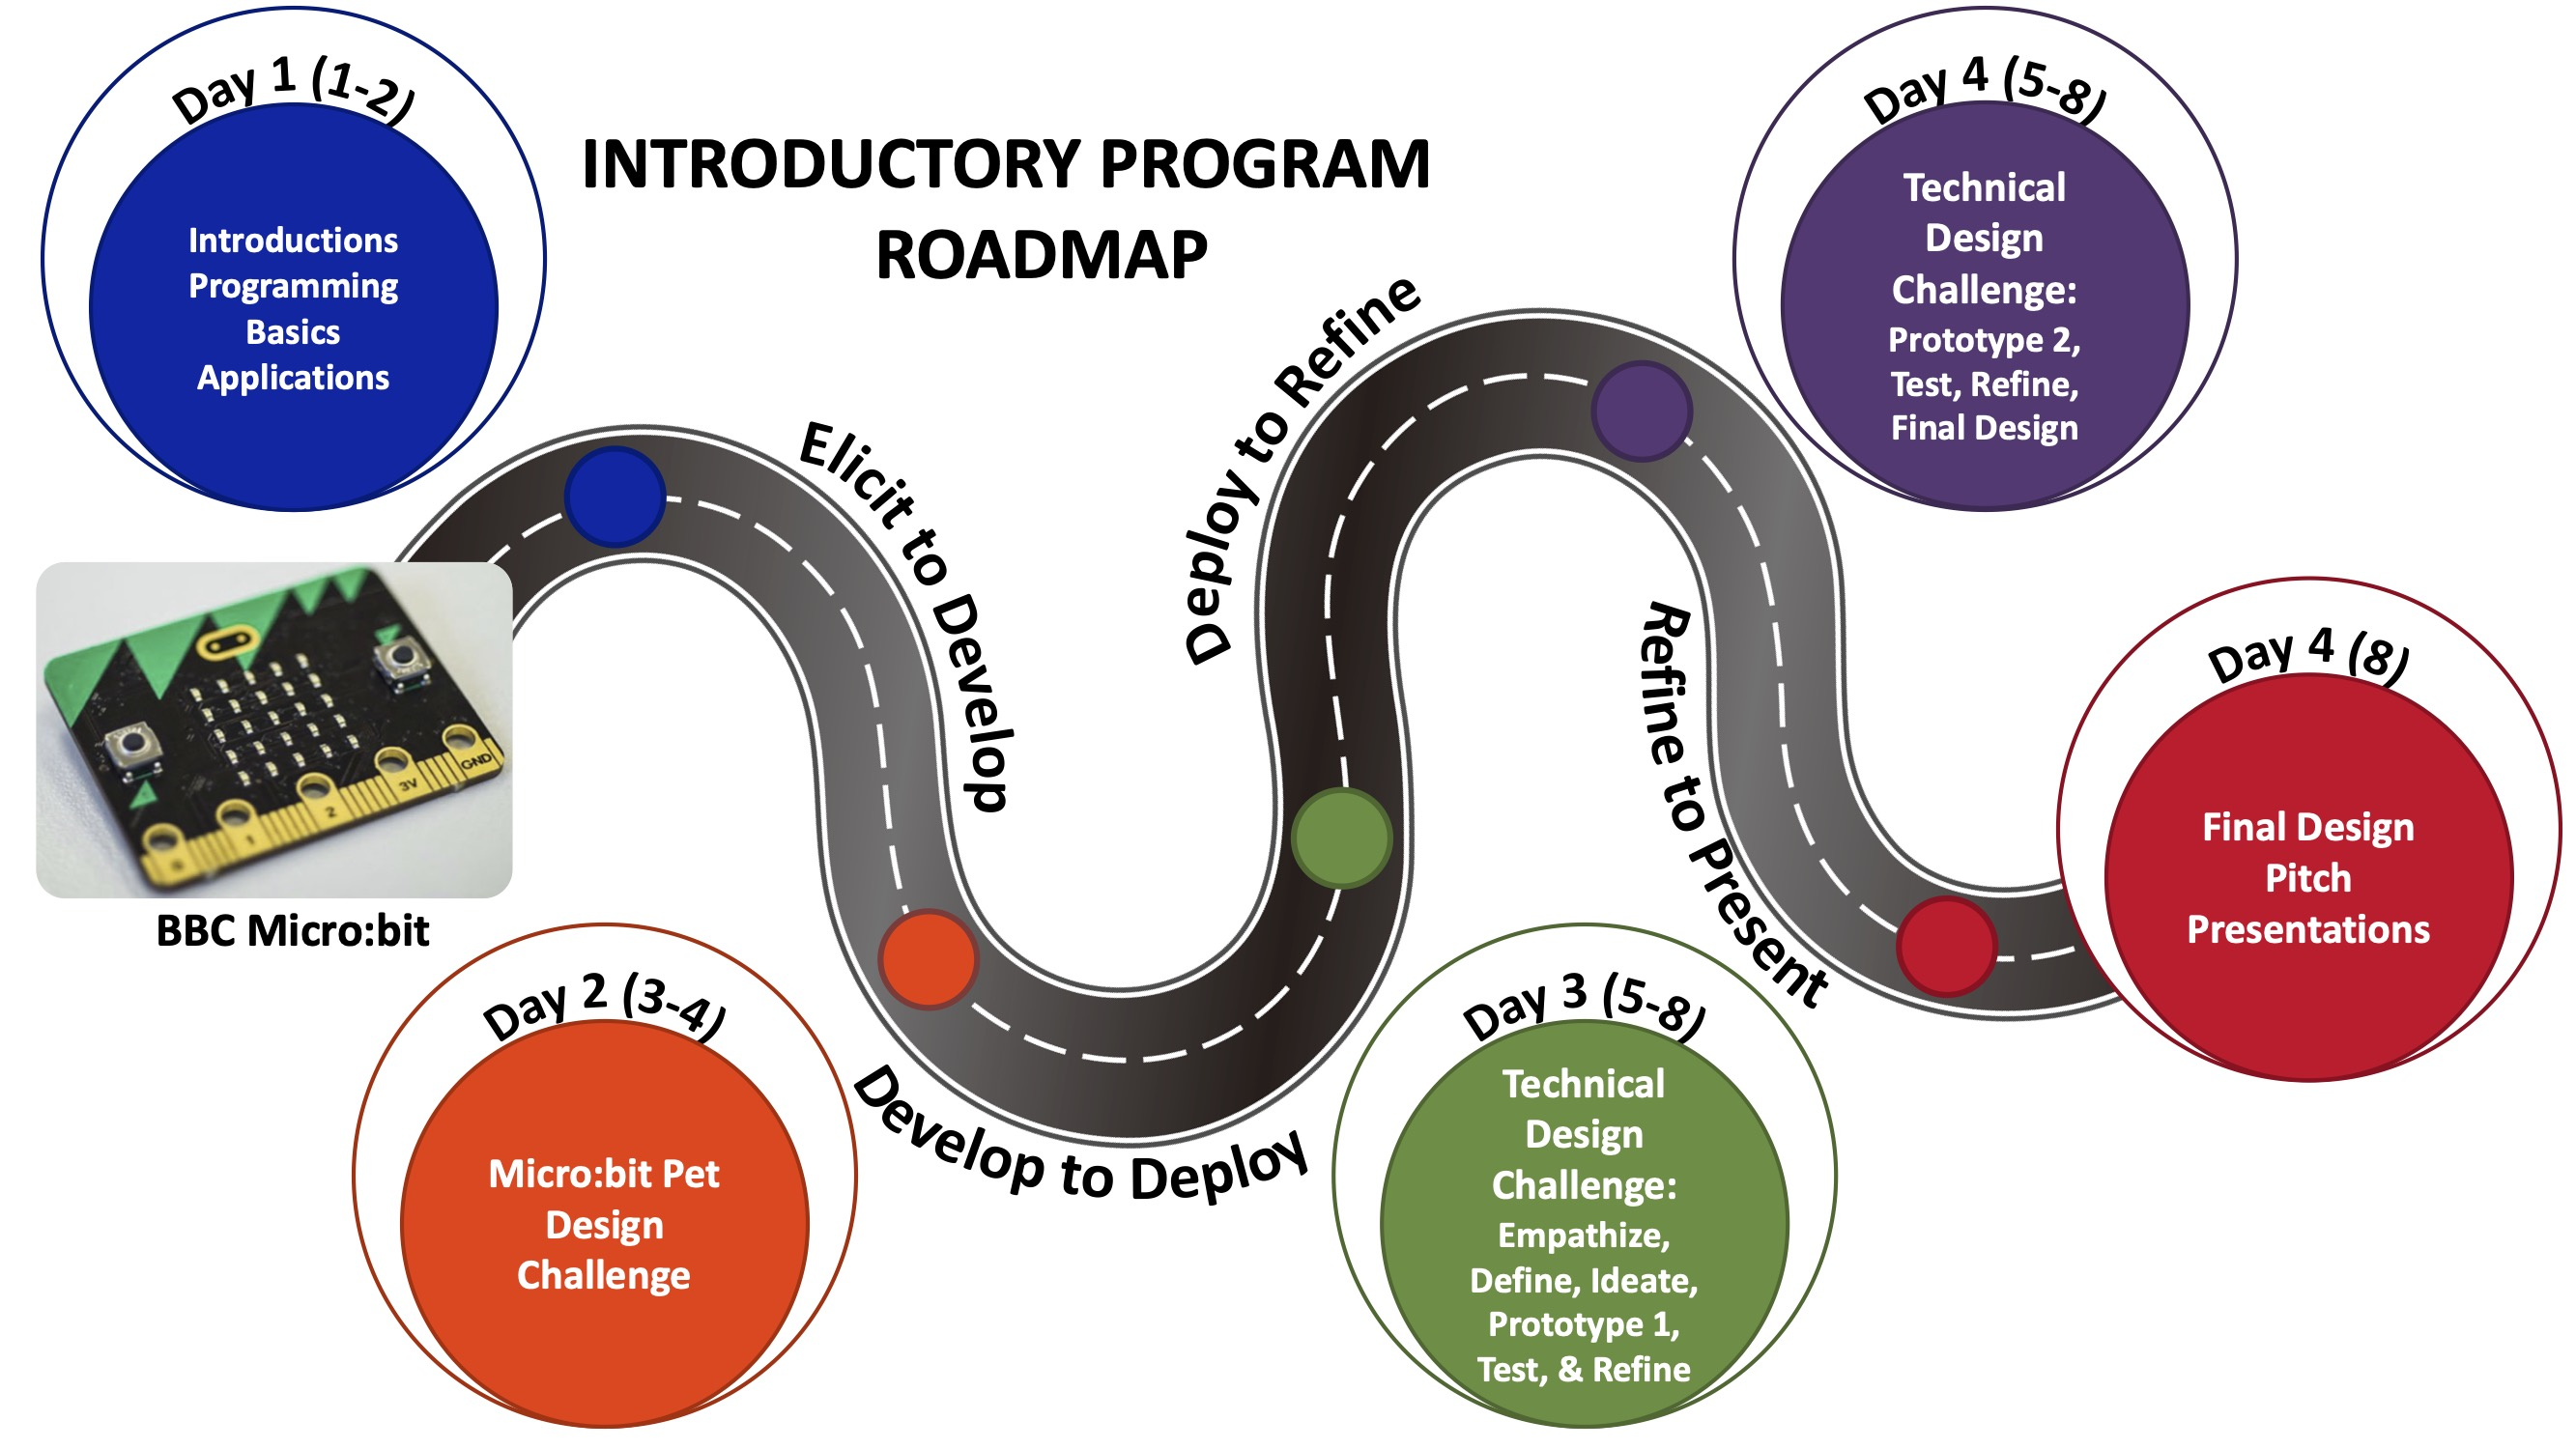
\includegraphics[width=0.8\textwidth,height=\textheight]{Images/GGEE_23_intro_roadmap.jpg}
\caption{\emph{Introductory Program Roadmap}}
\end{figure}

\hypertarget{advanced-programs}{%
\subsection{Advanced Programs}\label{advanced-programs}}

The Advanced Program was formatted as 4 day program in all the pilot
schools, Figure \^{}. On Day 1, Students were introduced to the basic
concepts of artificial intelligence and then machine learning. The day
was concluded with an introduction to programming in
\href{https://scratch.mit.edu/}{Scratch} to prepare for the following
day.

On Day 2, students were introduced to Image-based and Test-based machine
learning models from
\href{https://machinelearningforkids.co.uk/}{Machine Learning for Kids}.
Classrooms were set up and students were given a login and password
unique to their session location. Students develop and train a
image-based machine learning model that analyzes the color
characteristics of different types of Pokémon. Students then build and
train a text-based machine learning model to develop a smart classroom
with electronic devices that power on or off using a variety of
commands.

On Day 3, students use their micro:bit programming skills from the
previous summer program combined with their new machine learning skills
to program a micro:bit to be able to identify different types of
gestures. During this activity, students built their own sets of
training data using the micro:bits. Students would program 2 gestures
together as a class and then make up to 5 gestures on their own. There
were at least 20-30 data points for each gesture. The machine learning
models were trained using a decision tree constructed in Python and
hosted in a Juypter Notebook on \href{https://nanohub.org/}{NanoHub}.
The model was loaded onto the micro:bit and the model would identify
gestures based on the training data provided.

On Day 4, students were introduced to Neural Networks. The activity
walked them through the various types of machine learning models from
decision trees to more complex neural networks. Students learned about
the multiple layers in a neural network and the processes that each of
those layer serve. The following activity had students develop and train
a neural network to identify images of numbers. Students manipulated the
number of nodes and studied the effect on the outcame and weights in
identifying each number. This activity concluded the program.

\begin{figure}
\centering
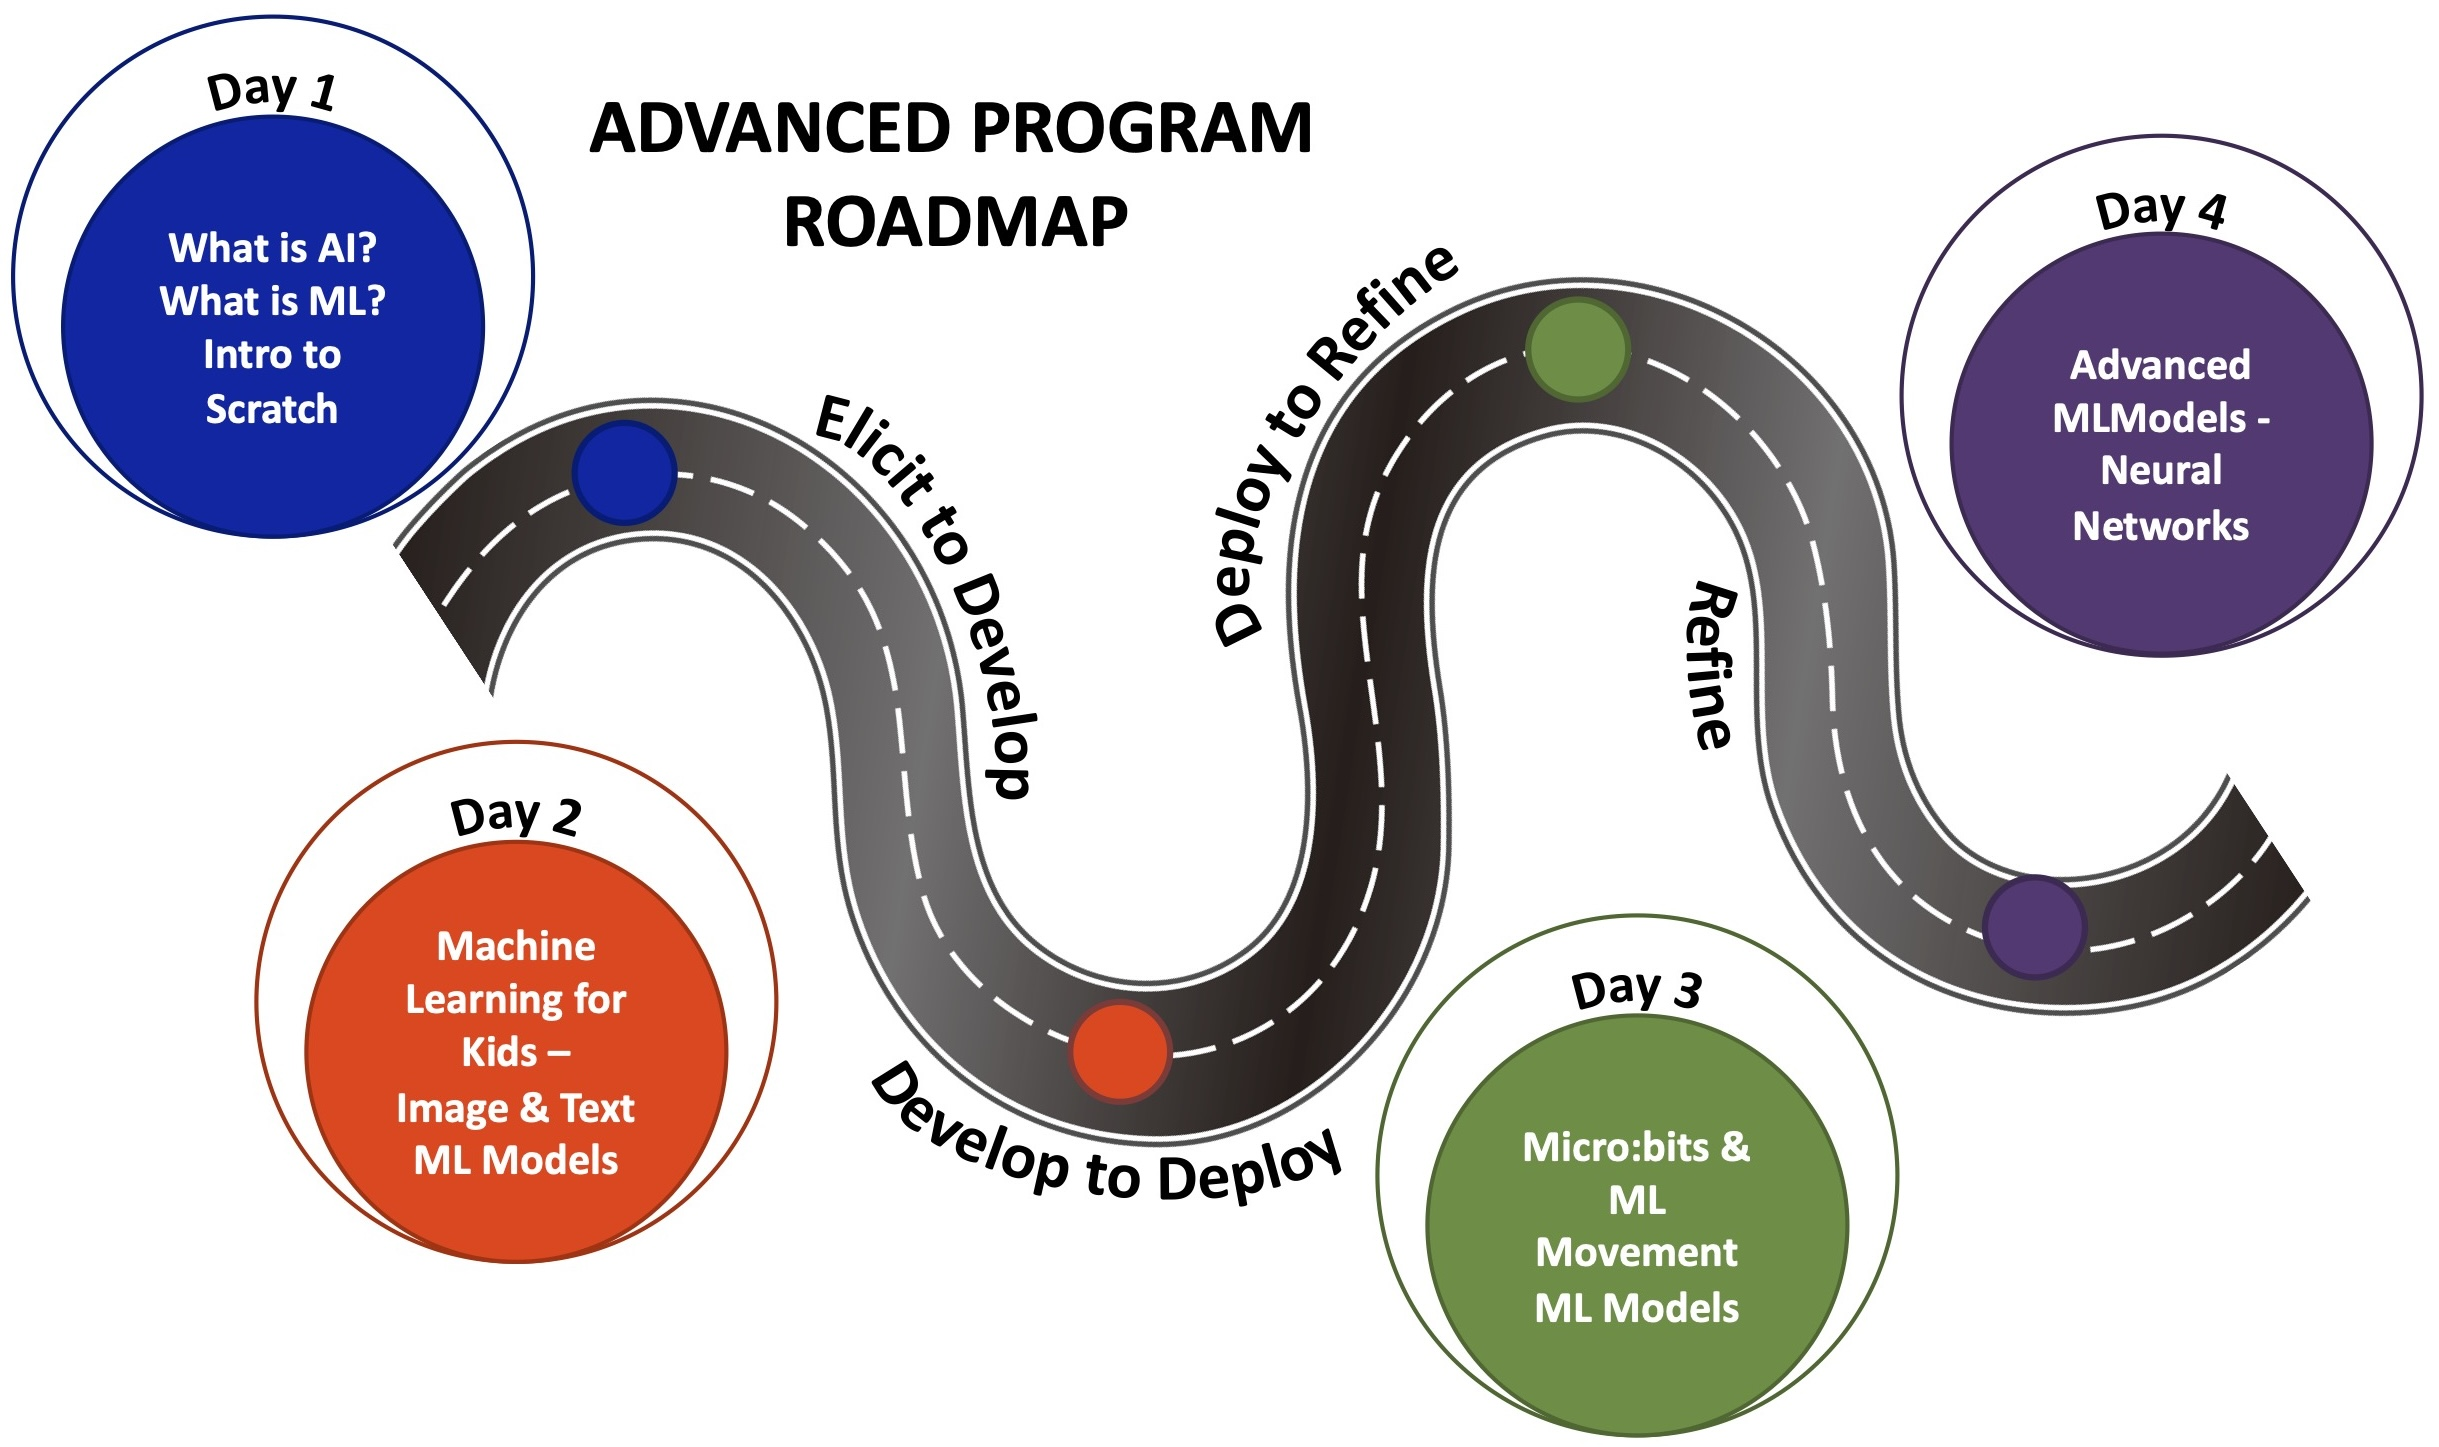
\includegraphics[width=0.8\textwidth,height=\textheight]{Images/GGEE_23_Adv_roadmap.jpg}
\caption{\emph{Advanced Program Roadmap}}
\end{figure}

\hypertarget{day-programs}{%
\subsection{4-Day Programs}\label{day-programs}}

\hypertarget{day-programs-1}{%
\subsection{8-Day Programs}\label{day-programs-1}}

\hypertarget{student-enrollment-demographics}{%
\section{Student Enrollment \&
Demographics}\label{student-enrollment-demographics}}

\hypertarget{enrollment-statistics}{%
\subsection{Enrollment Statistics}\label{enrollment-statistics}}

\emph{Present enrollment data, including the number of students who
initially registered, and any changes over the course of the program.}

Programs were able to host up to 25 students in each of their program
sessions. Registrations were closed and students were placed on wait
lists in the case of cancellations by student parents. Programs had on
average X number of students enroll. Wait lists ranged from 5 - 80
students in some districts.

Bar Graph Comparison - Total Number of Registered Students - stacked bar
graph - registered vs waitlist

\textbf{GRAPH by Session - stacked graph - regsitered vs waitlist}

Need for more programs in Santa Rosa County District Schools

\hypertarget{attendance-records}{%
\subsection{Attendance Records}\label{attendance-records}}

\emph{Share attendance records to illustrate the level of student
engagement and participation throughout the program.}

Actual attendance with the programs were less than initial
registrations. Students became ill, were unable to attend the first days
of the program or parents made new plans for their families.

\begin{figure}
\centering
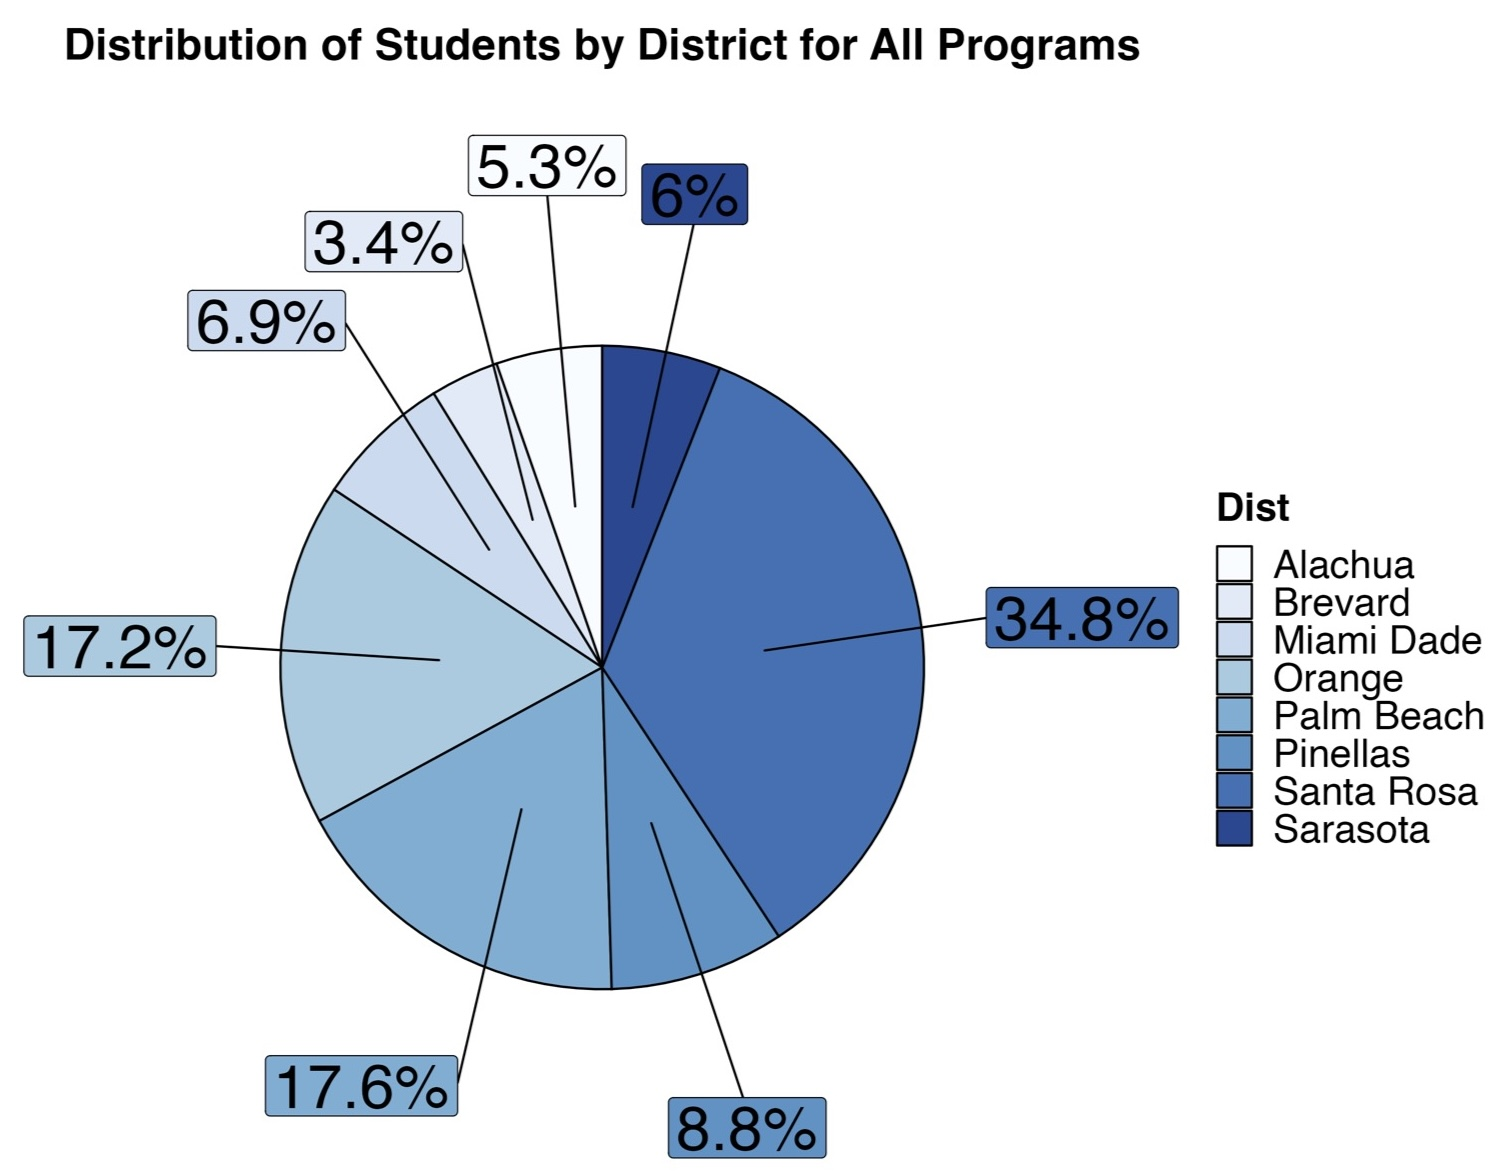
\includegraphics[width=0.55\textwidth,height=\textheight]{Graphs/Report/GGEE_23_District_All.jpg}
\caption{\emph{The percentage of students by district for both
introductory and advanced Goldberg Gator Engineering Explorer Summer
Programs (n=319)}}
\end{figure}

\begin{figure}
\centering
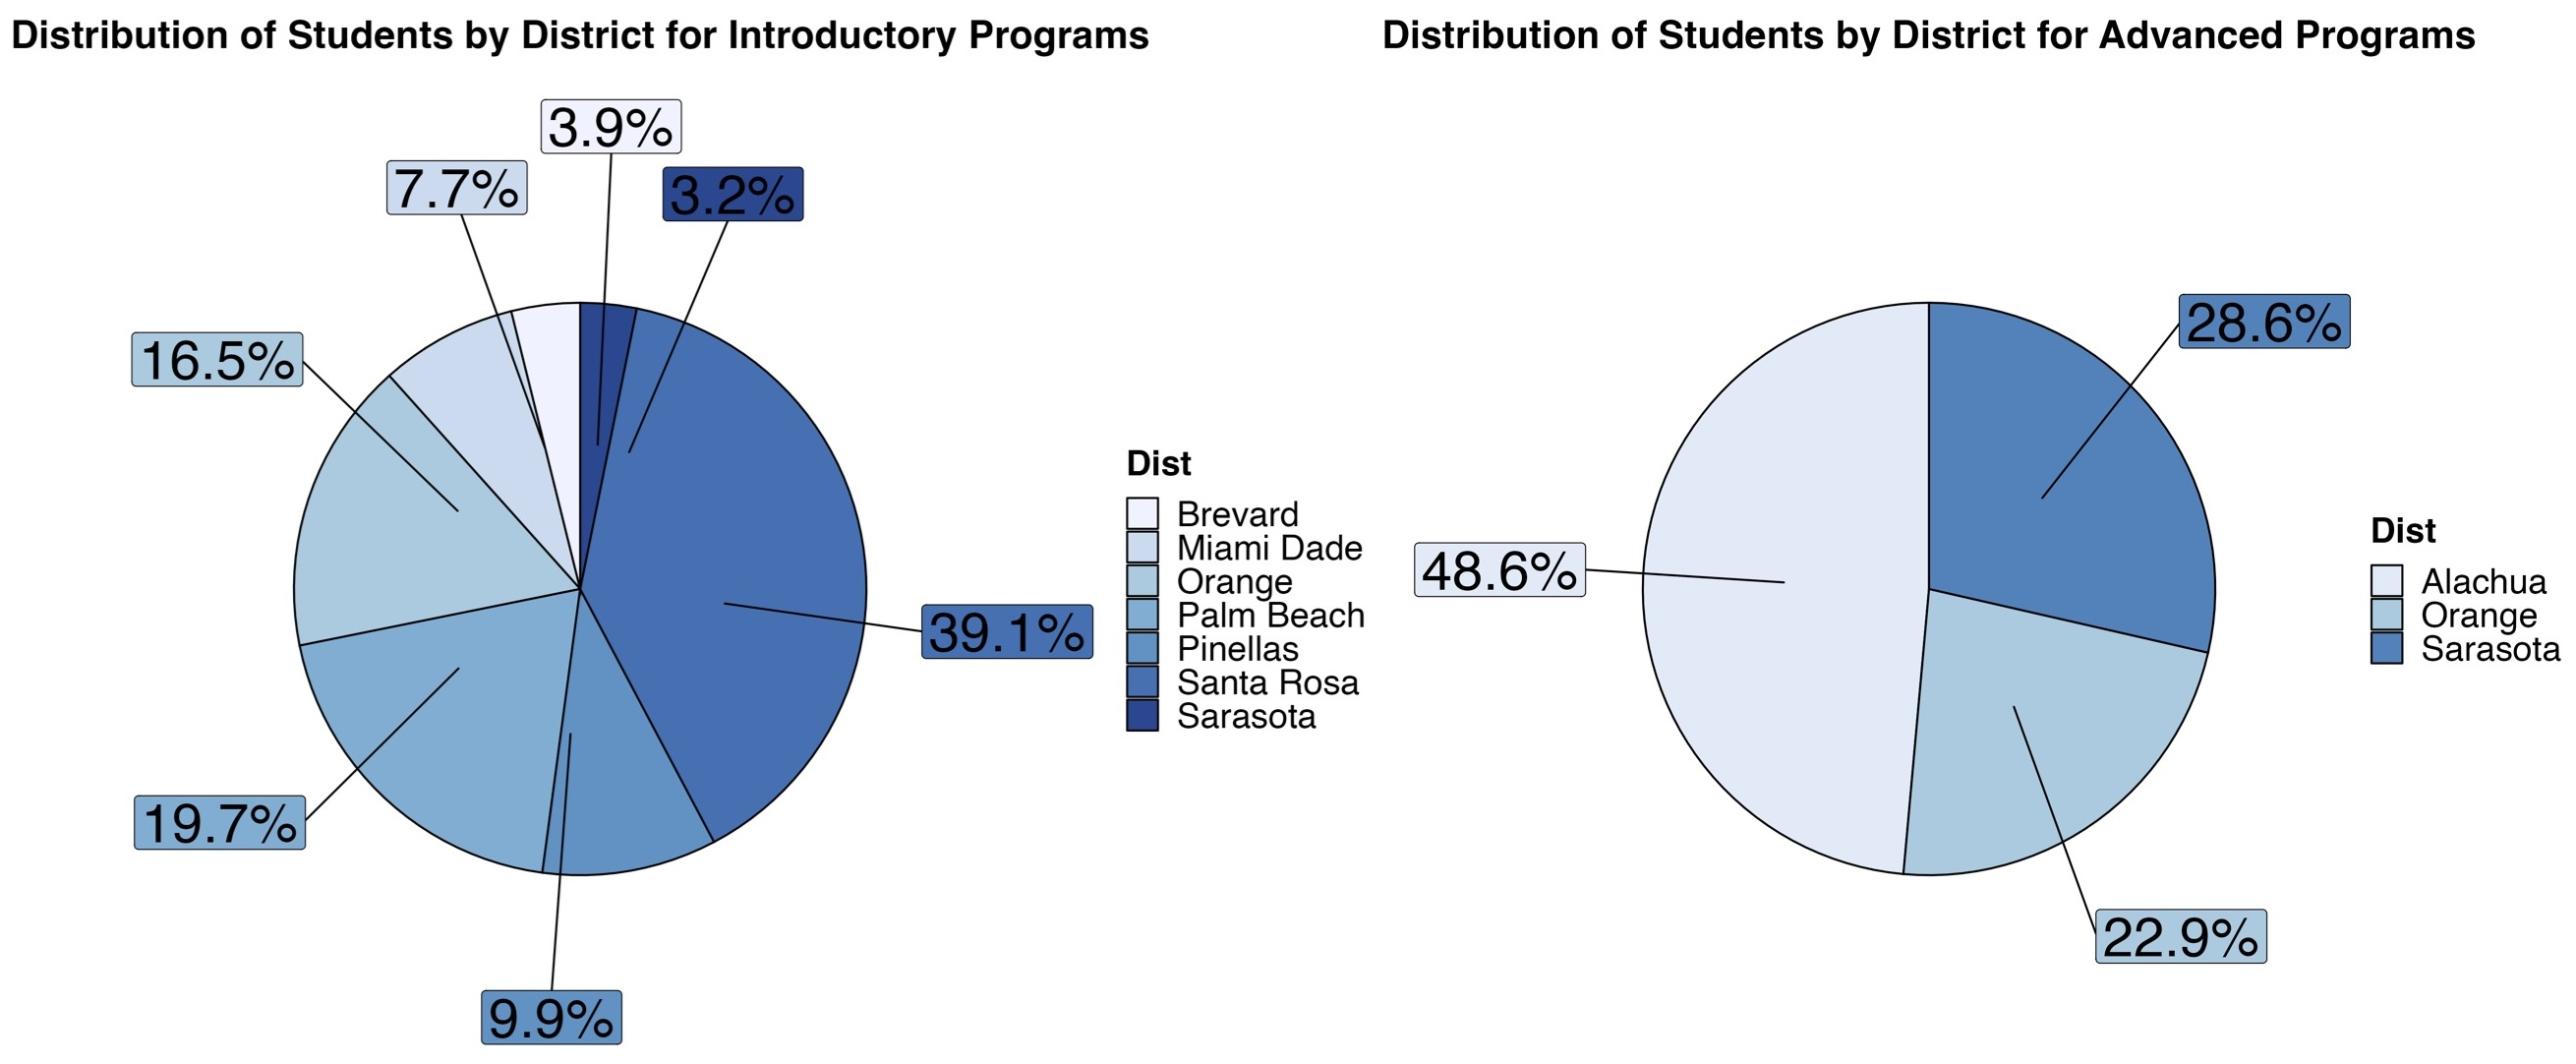
\includegraphics{Graphs/Report/GGEE_23_District_IA.jpg}
\caption{\emph{The percentage of students by district for the
introductory (left, n=284) and advanced (right,n=35) Goldberg Gator
Engineering Explorer Summer Programs}}
\end{figure}

\hypertarget{student-demographics}{%
\subsection{Student Demographics}\label{student-demographics}}

Demographics were collected from students that participated in the
resaerch study. There were a total of 204 students that participated in
the GGEE Summer programs. \textbf{add amounts from intro and advanced}

\hypertarget{age}{%
\subsubsection{Age}\label{age}}

\emph{Include demographic information such as age, gender, ethnicity,
and socioeconomic background of the participating students.}

\begin{figure}
\centering
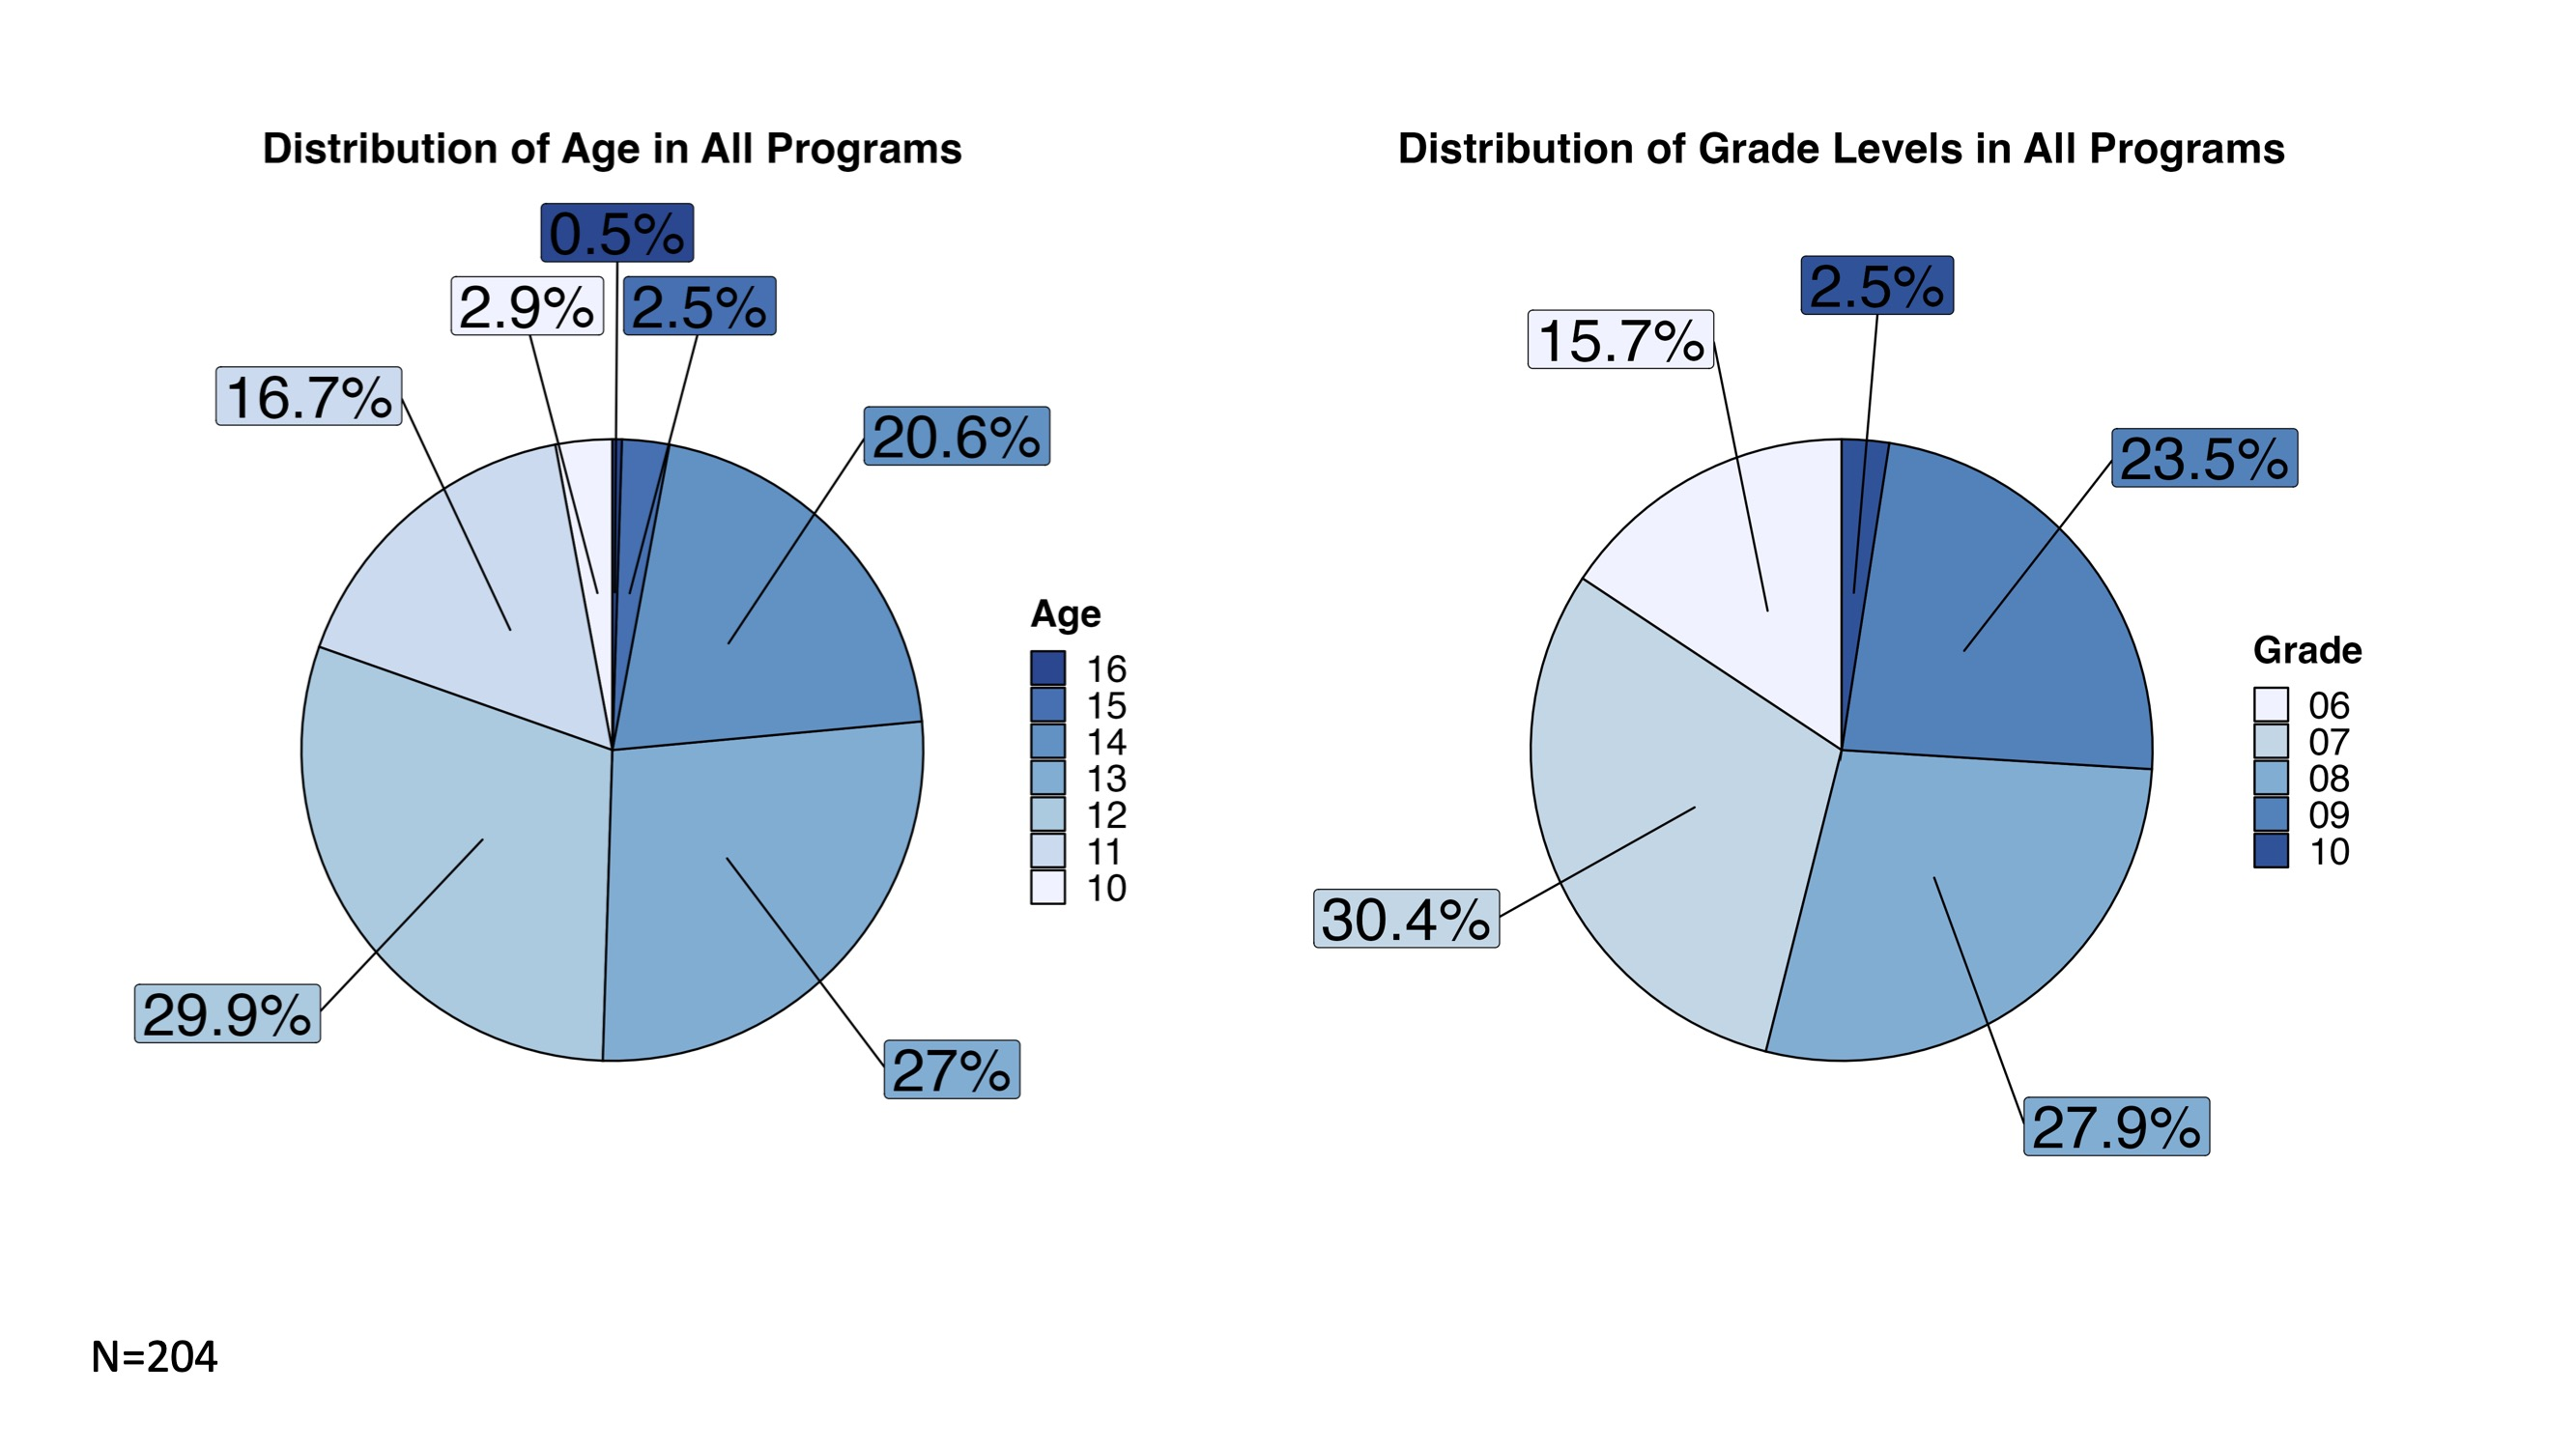
\includegraphics[width=0.45\textwidth,height=\textheight]{Graphs/Report/GGEE_23_Age_All.jpg}
\caption{\emph{The percentage of student age for both introductory and
advanced Goldberg Gator Engineering Explorer Summer Programs (n=204)}}
\end{figure}

\begin{figure}
\centering
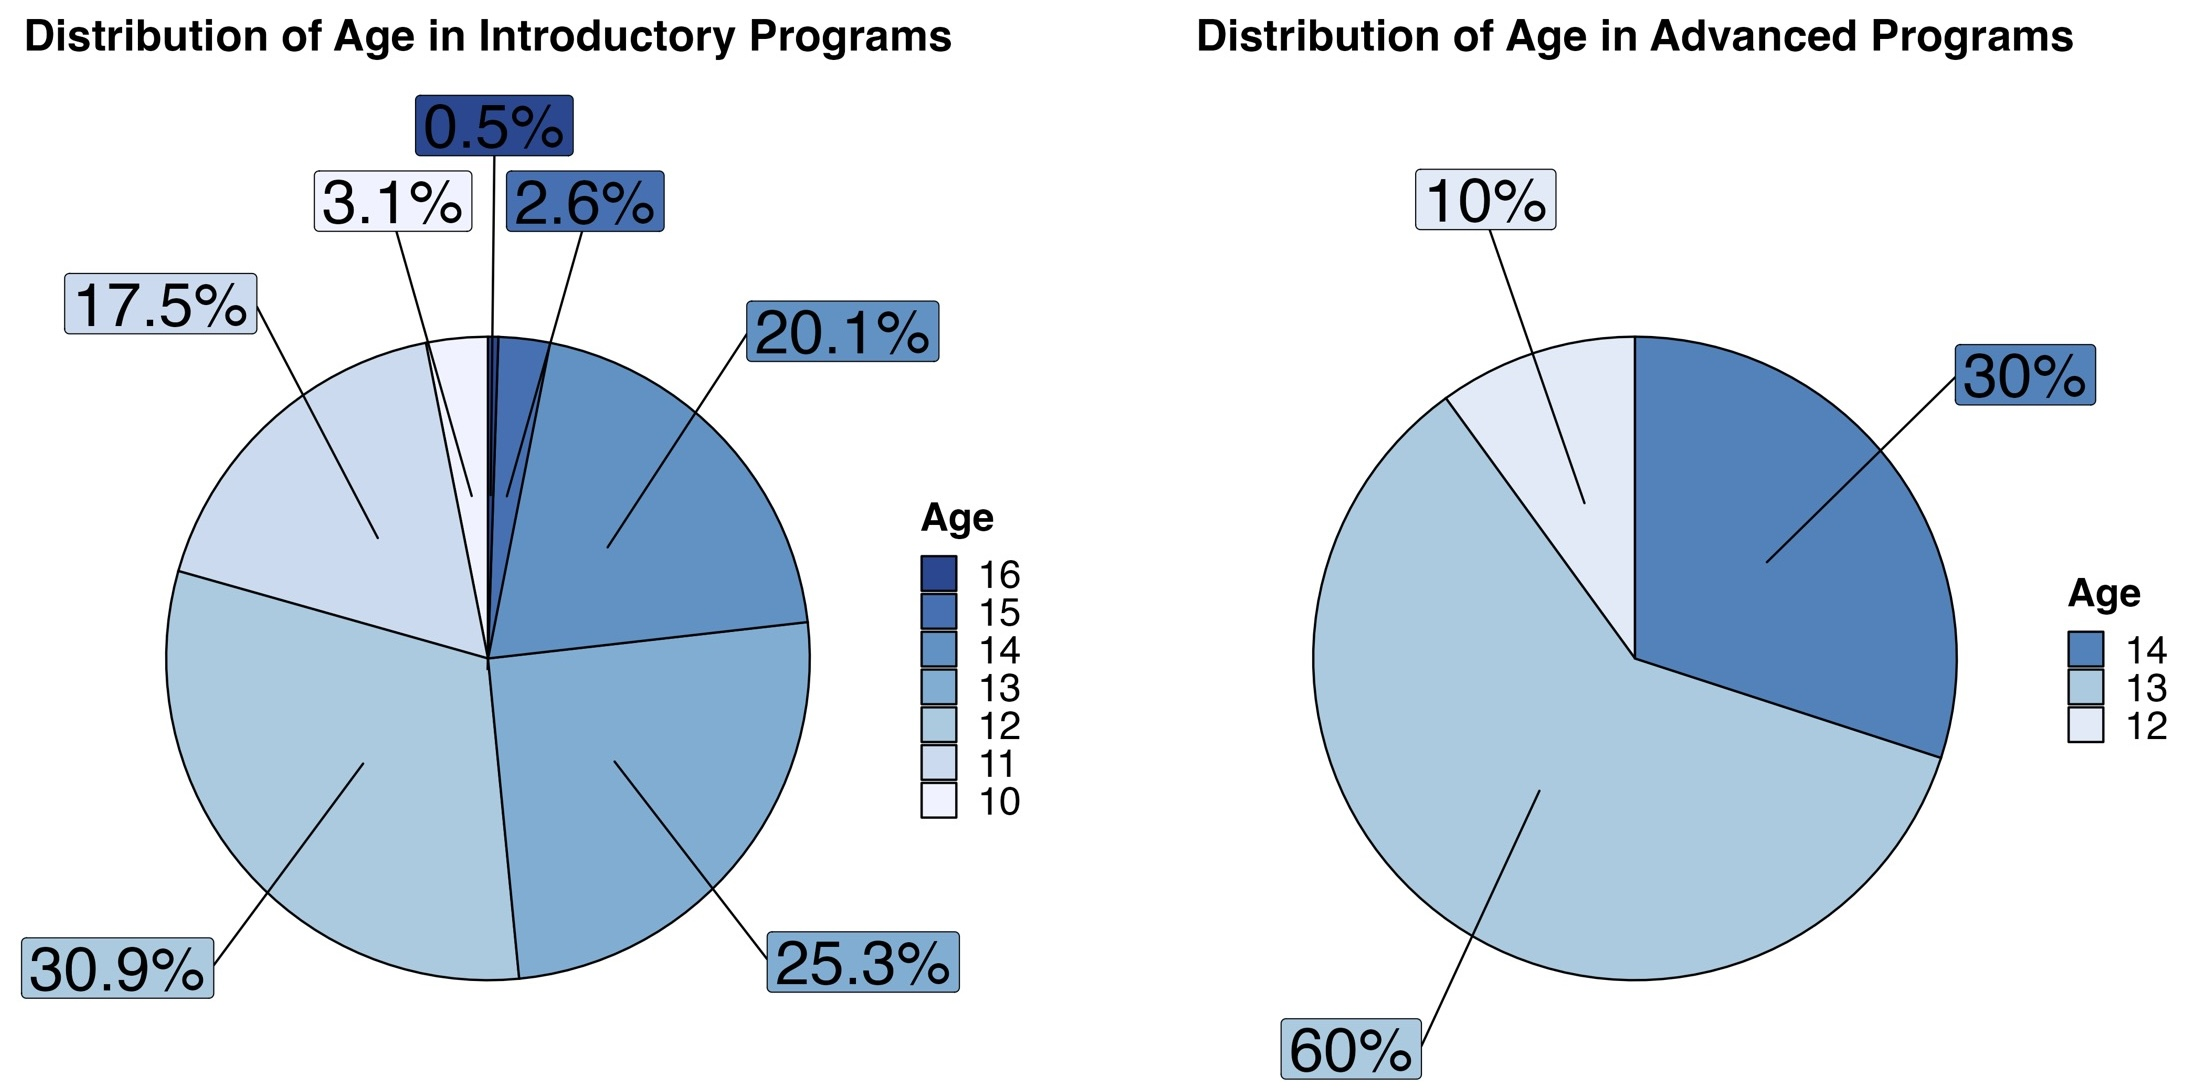
\includegraphics[width=0.85\textwidth,height=\textheight]{Graphs/Report/GGEE_23_Age_IA.jpg}
\caption{\emph{The percentage of students ages for the introductory
(left, n=194) and advanced (right,n=10) Goldberg Gator Engineering
Explorer Summer Programs}}
\end{figure}

\hypertarget{gender}{%
\subsubsection{Gender}\label{gender}}

\begin{figure}
\centering
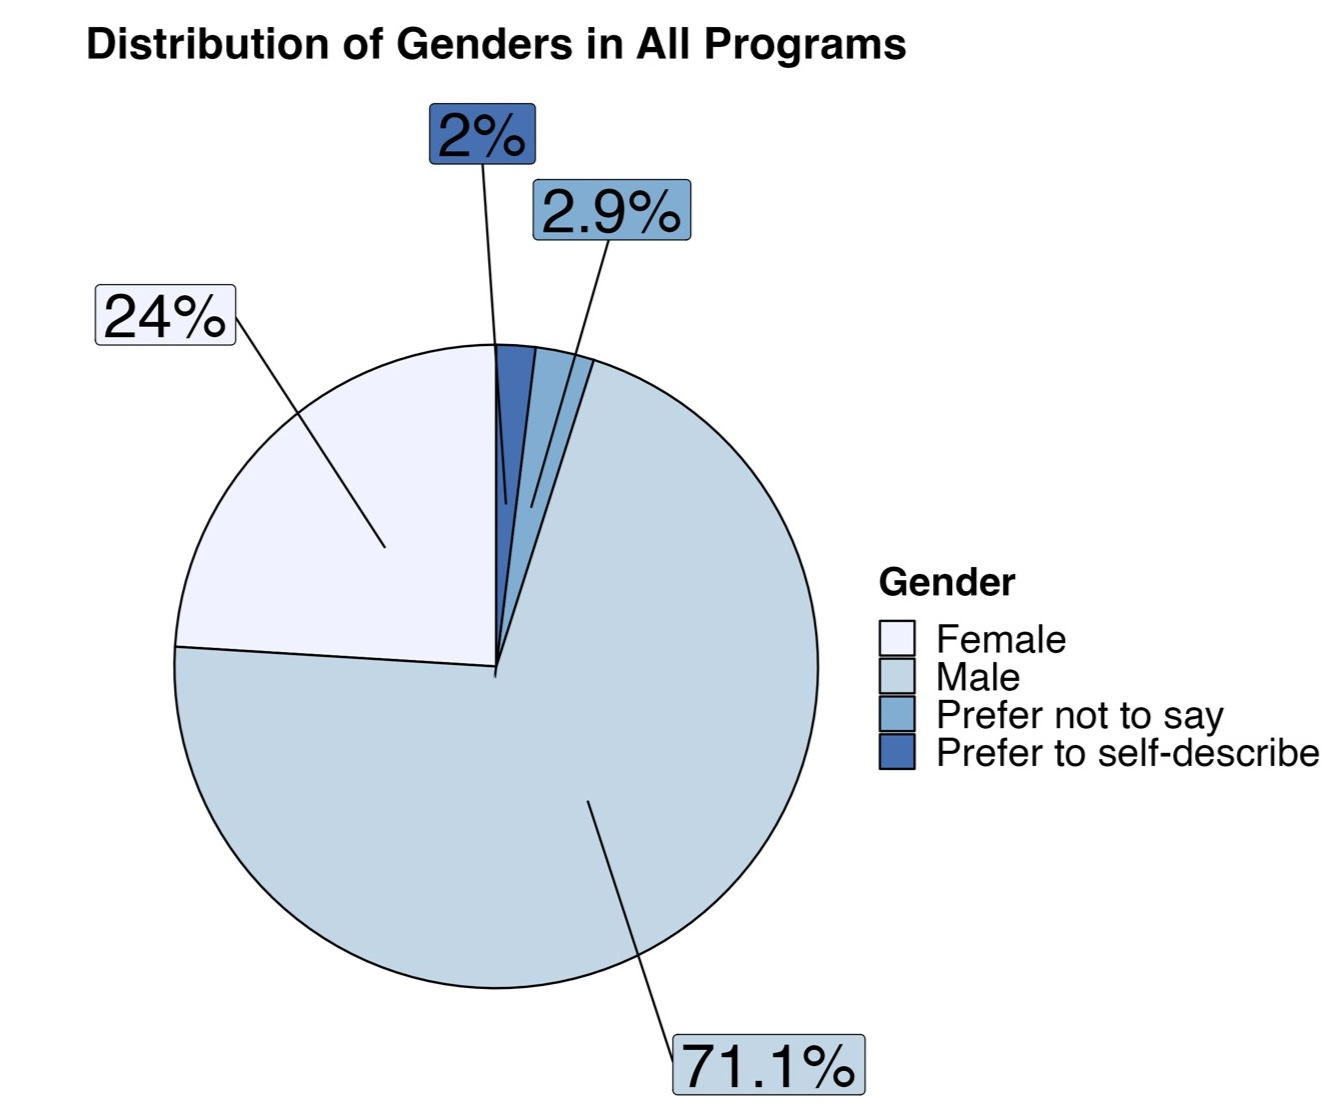
\includegraphics[width=0.5\textwidth,height=\textheight]{Graphs/Report/GGEE_23_Gender_All.jpg}
\caption{\emph{The percentage of student genders for both introductory
and advanced Goldberg Gator Engineering Explorer Summer Programs
(n=204)}}
\end{figure}

\begin{figure}
\centering
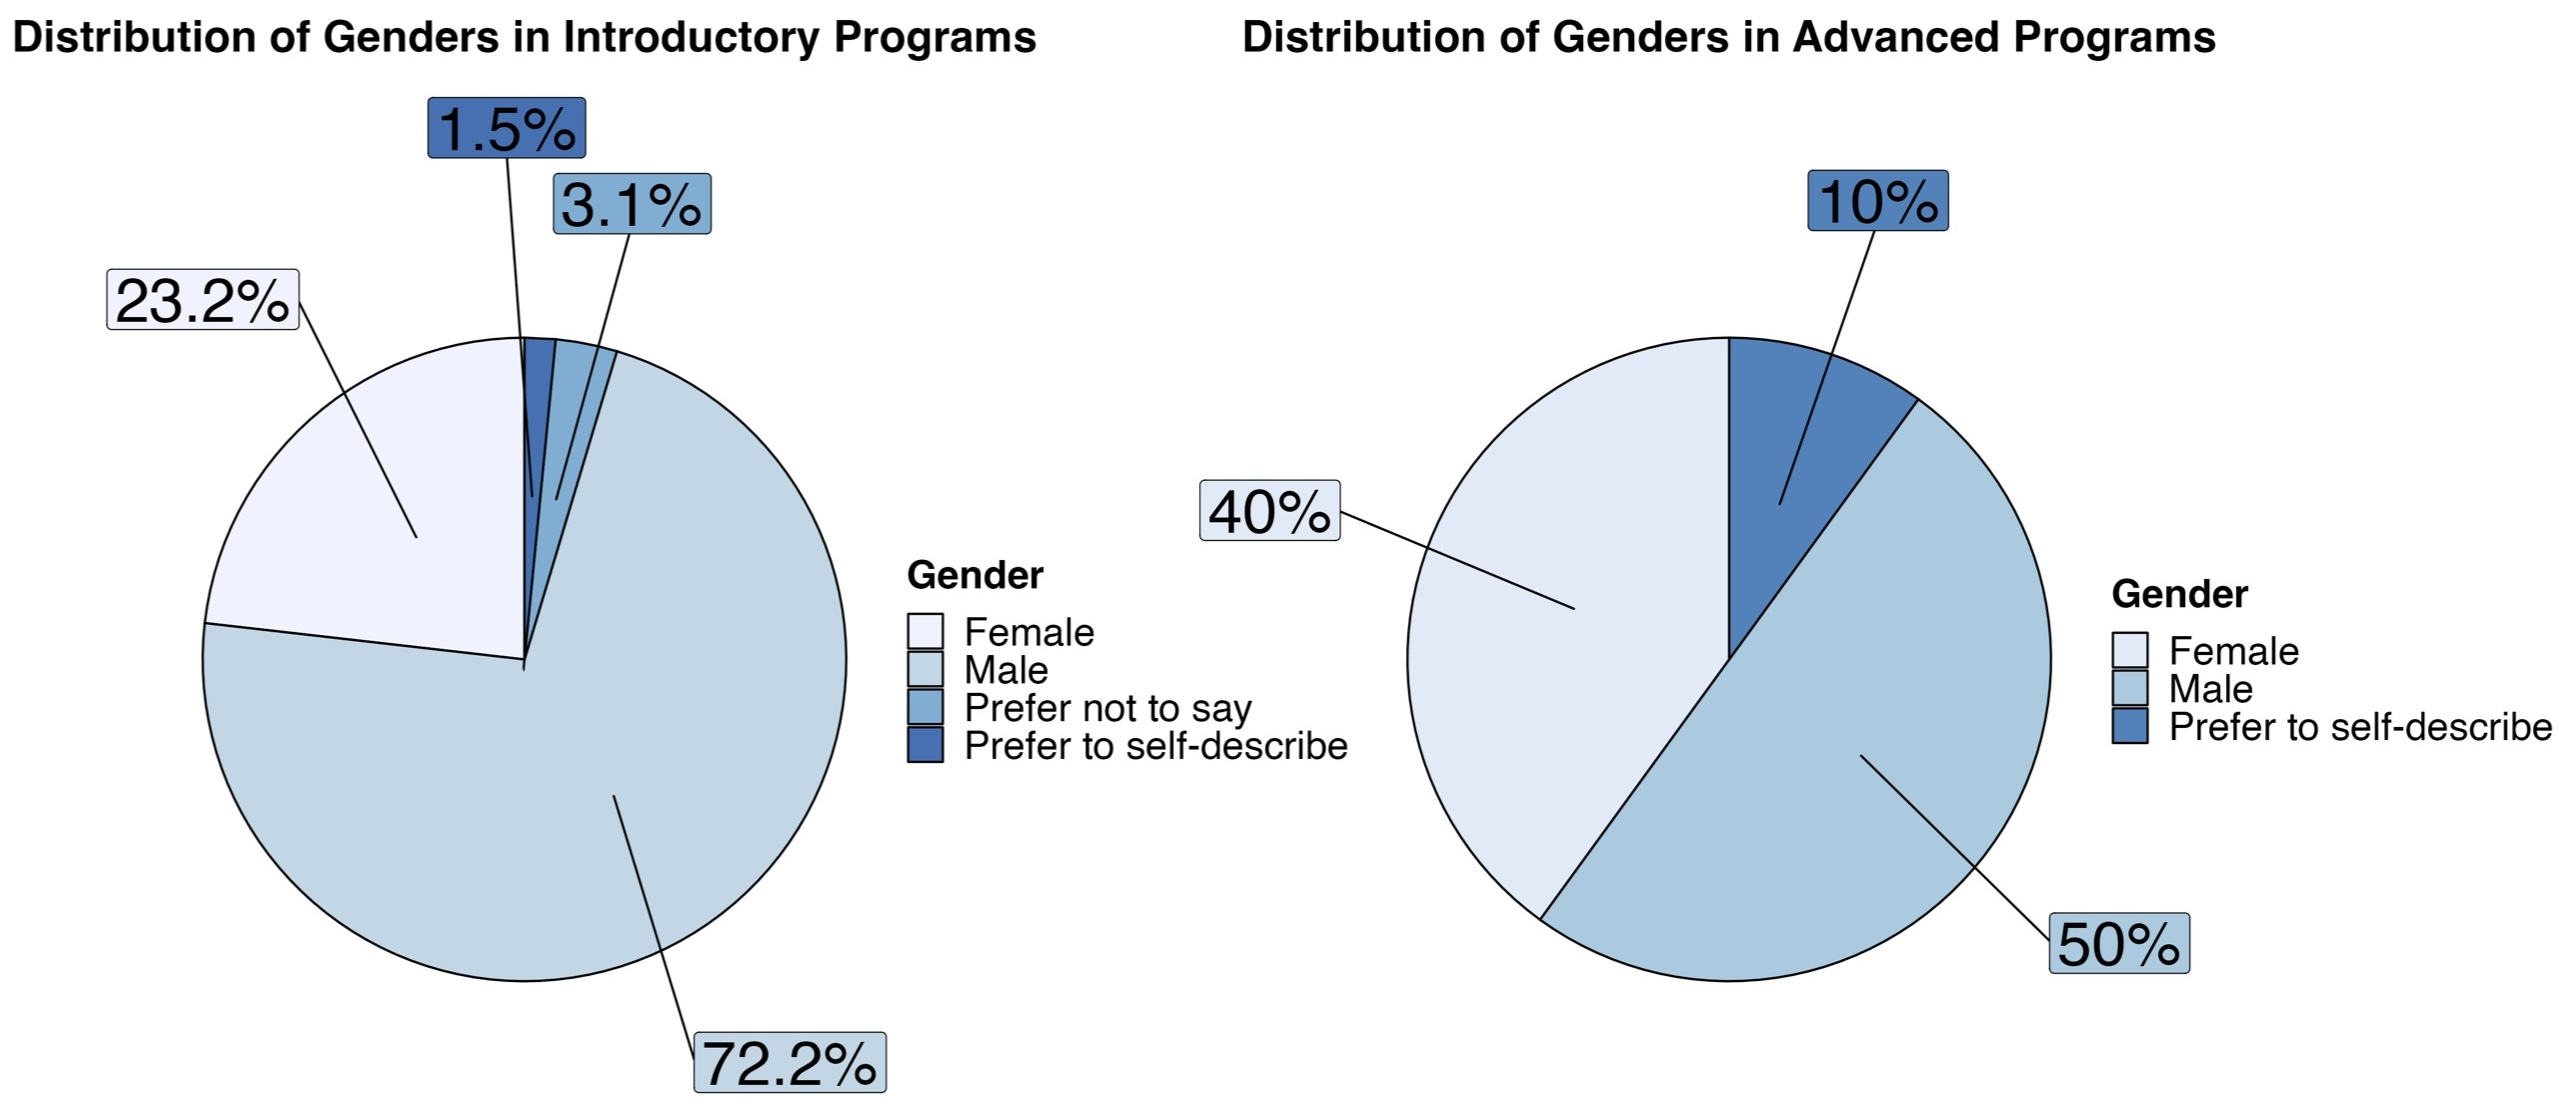
\includegraphics{Graphs/Report/GGEE_23_Gender_IA.jpg}
\caption{\emph{The percentage of students genders for the introductory
(left, n=194) and advanced (right,n=10) Goldberg Gator Engineering
Explorer Summer Programs}}
\end{figure}

\hypertarget{race-and-ethnicity}{%
\subsubsection{Race and Ethnicity}\label{race-and-ethnicity}}

\begin{itemize}
\tightlist
\item
  Students that chose 3 or more race and ethnicity were grouped together
\item
  Count of students by race or ethnicity in each course
\item
  Many students selected multiple races or ethnicity, primary race with
  secondary ethniticty was listed
\item
  Broken down into percentage of secondary race or ethnicity
\end{itemize}

\begin{figure}
\centering
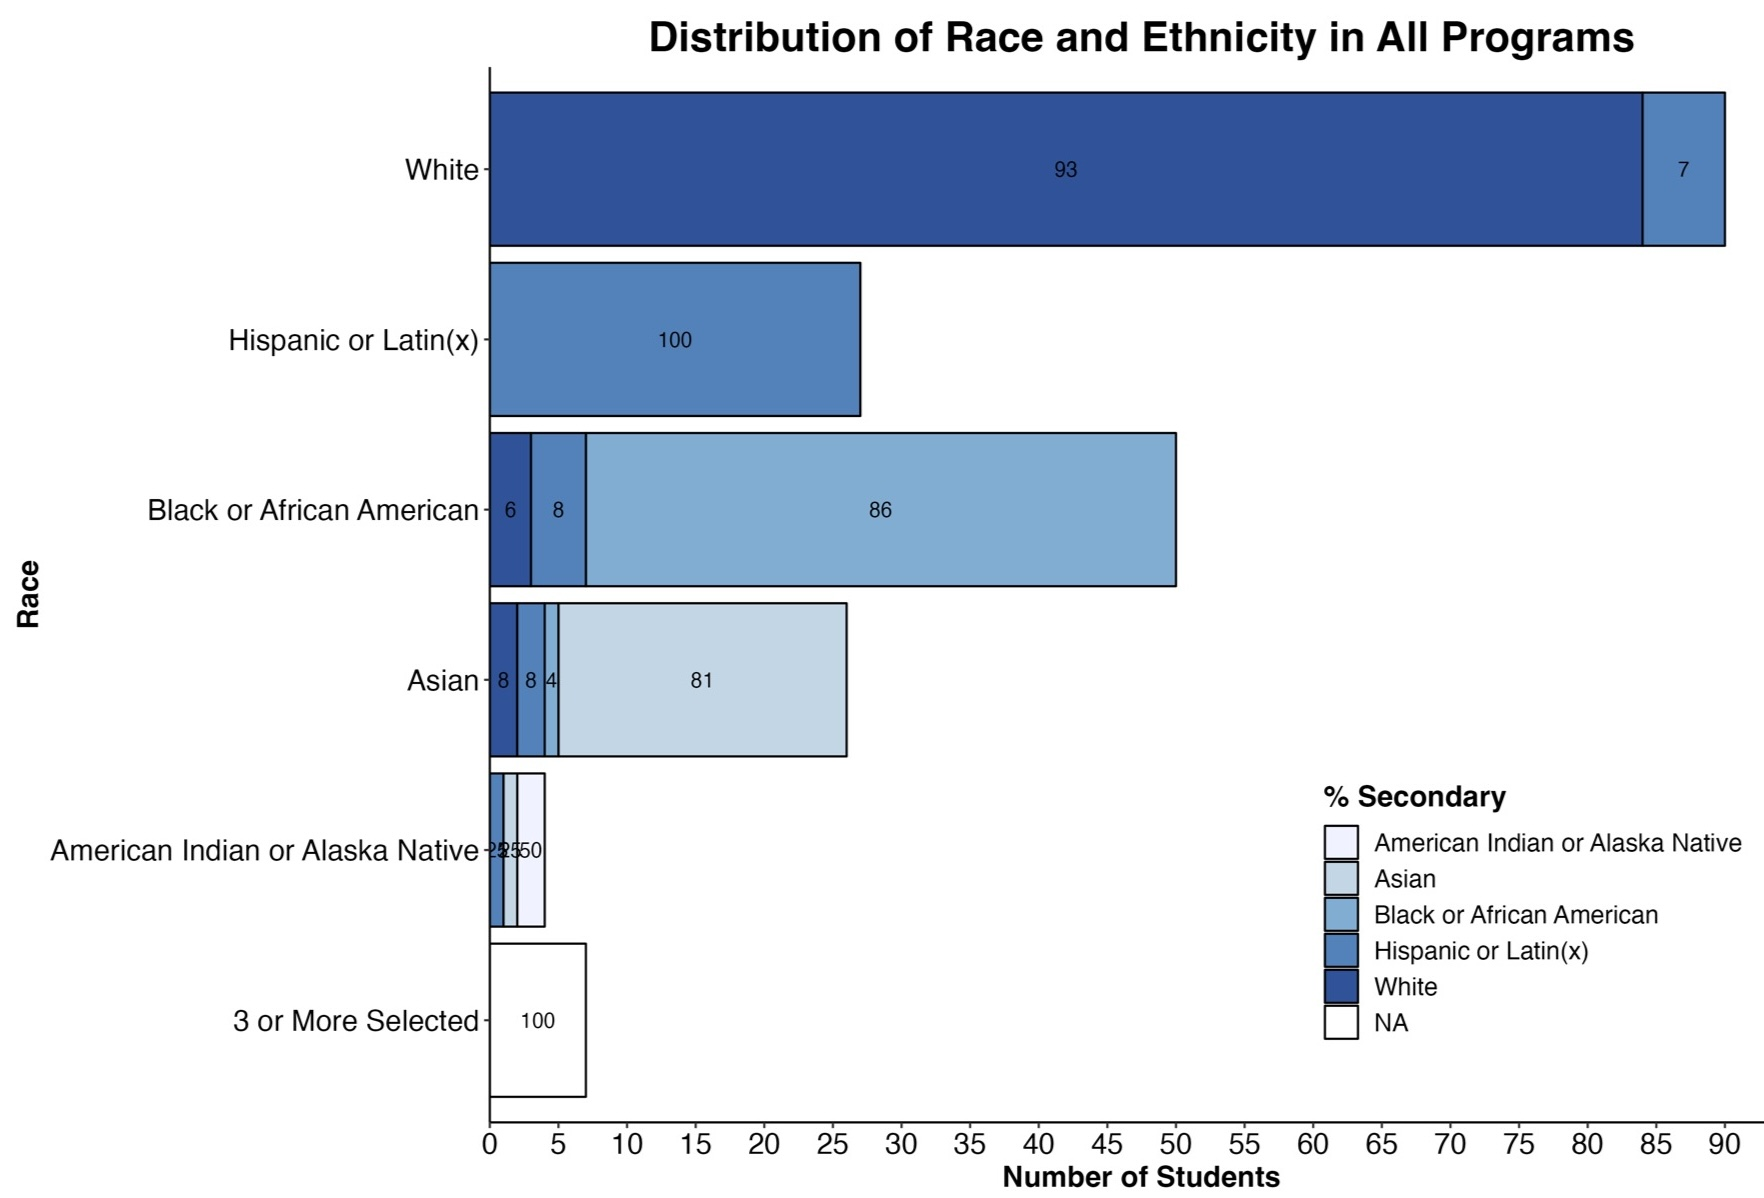
\includegraphics[width=0.8\textwidth,height=\textheight]{Graphs/Report/GGEE_23_Race_All.jpg}
\caption{\emph{The percentage of student race and ethnicities for both
introductory and advanced Goldberg Gator Engineering Explorer Summer
Programs (n=204)}}
\end{figure}

\begin{figure}
\centering
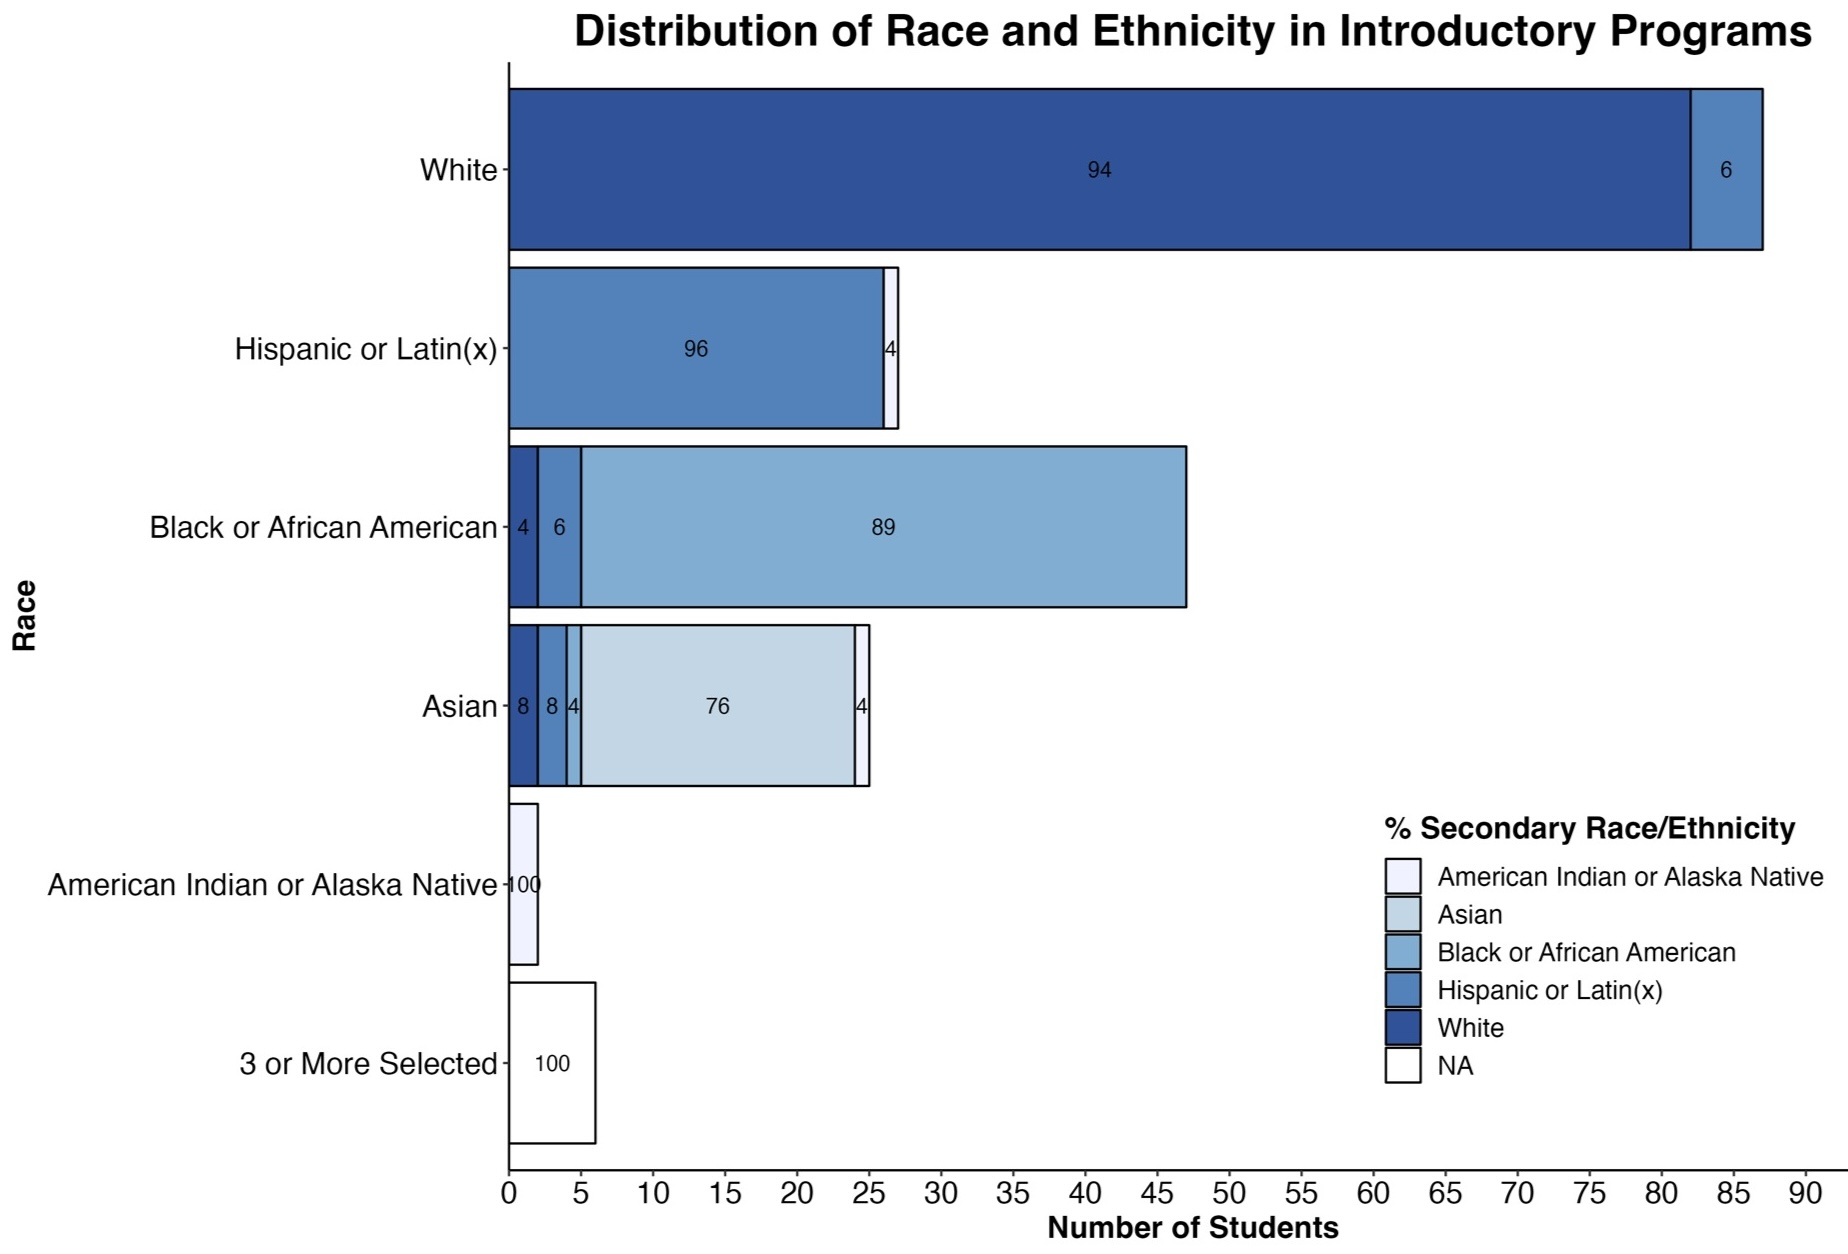
\includegraphics[width=0.8\textwidth,height=\textheight]{Graphs/Report/GGEE_23_Race_In.jpg}
\caption{\emph{The percentage of student race and ethnicities for
Introductory Goldberg Gator Engineering Explorer Summer Programs
(n=194)}}
\end{figure}

\begin{figure}
\centering
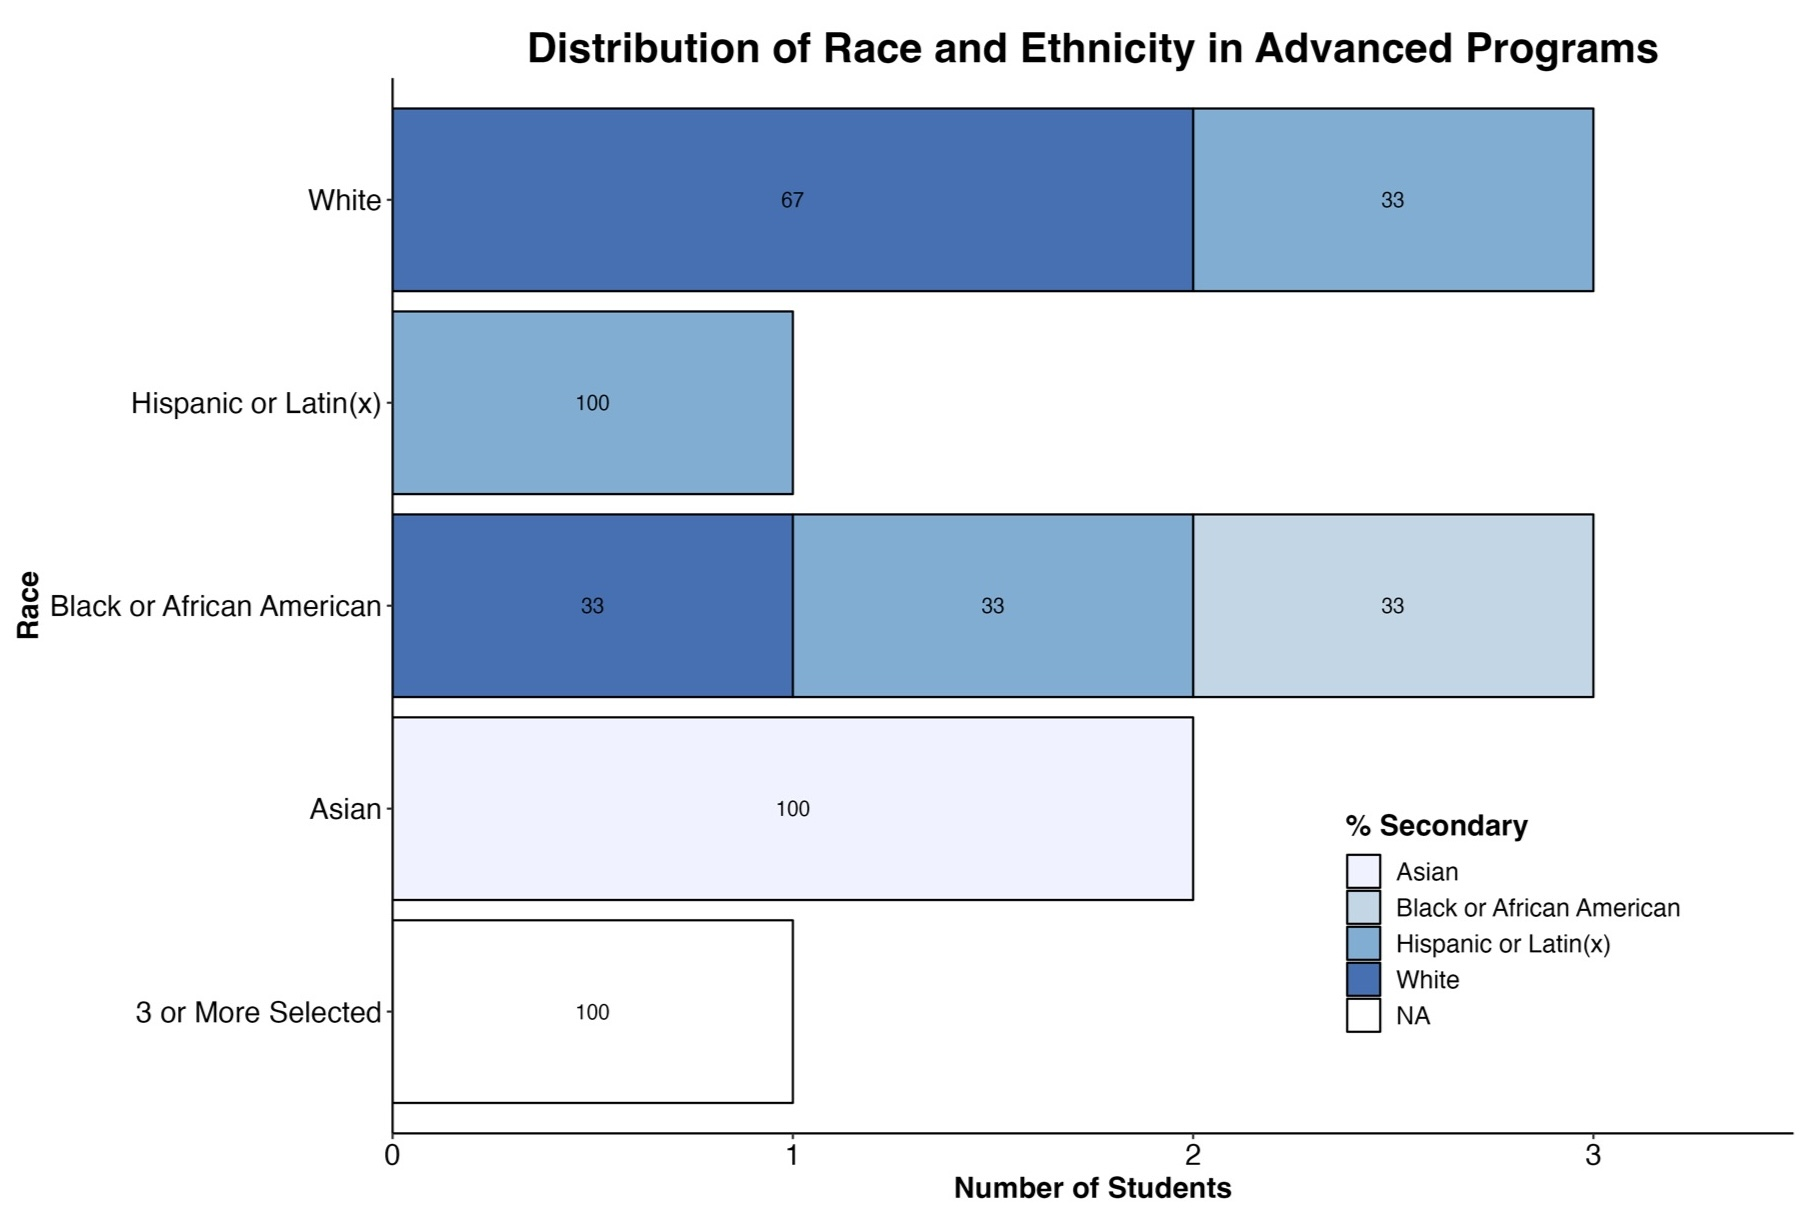
\includegraphics[width=0.8\textwidth,height=\textheight]{Graphs/Report/GGEE_23_Race_Adv.jpg}
\caption{\emph{The percentage of student race and ethnicities for
Advanced Goldberg Gator Engineering Explorer Summer Programs (n=10)}}
\end{figure}

\hypertarget{research-1}{%
\section{Research}\label{research-1}}

\hypertarget{summary-of-pre-survey-survey-results}{%
\subsection{Summary of Pre-Survey Survey
Results}\label{summary-of-pre-survey-survey-results}}

Summarize the responses from the pre-program survey, highlighting key
findings and insights.

\hypertarget{survey-responses}{%
\subsection{Survey Responses}\label{survey-responses}}

\hypertarget{analysis-of-ongoing-survey-data-if-conducted-during-the-program}{%
\subsection{Analysis of Ongoing Survey Data (if conducted during the
program)}\label{analysis-of-ongoing-survey-data-if-conducted-during-the-program}}

If you conducted surveys during the program, analyze the responses and
share any noteworthy trends or changes over time.

\hypertarget{student-interviews}{%
\subsection{Student Interviews}\label{student-interviews}}

\hypertarget{highlights-from-student-interviews}{%
\subsubsection{Highlights from Student
Interviews}\label{highlights-from-student-interviews}}

Share significant insights and quotes gathered from student interviews,
emphasizing their experiences and perspectives.

\hypertarget{end-of-program-survey-responses}{%
\subsection{End of Program Survey
Responses}\label{end-of-program-survey-responses}}

\hypertarget{summary-of-post-program-survey-results}{%
\subsubsection{Summary of Post-Program Survey
Results}\label{summary-of-post-program-survey-results}}

Present the results of the post-program survey, emphasizing any changes
in student responses compared to the pre-program survey.

\hypertarget{program-outcomes}{%
\section{Program Outcomes}\label{program-outcomes}}

\hypertarget{assessment-of-program-objectives-and-goals}{%
\subsection{Assessment of Program Objectives and
Goals}\label{assessment-of-program-objectives-and-goals}}

Evaluate whether the program met its objectives and goals as outlined in
the introduction.

\hypertarget{challenges-and-lessons-learned}{%
\section{Challenges and Lessons
Learned}\label{challenges-and-lessons-learned}}

\hypertarget{identification-of-challenges-faced}{%
\subsection{Identification of Challenges
Faced}\label{identification-of-challenges-faced}}

Discuss any challenges encountered during the program's implementation.

\hypertarget{lessons-learned-adaptations-made}{%
\subsection{Lessons Learned \& Adaptations
Made}\label{lessons-learned-adaptations-made}}

Share lessons learned from the program's challenges and any adjustments
or improvements made as a result.

\hypertarget{recommendations}{%
\section{Recommendations}\label{recommendations}}

\hypertarget{suggestions-for-program-improvement}{%
\subsection{Suggestions for Program
Improvement}\label{suggestions-for-program-improvement}}

\emph{Provide recommendations for improving the program in future
iterations, based on the insights gained.}

\begin{itemize}
\tightlist
\item
  Updating compliance forms with more clear langaue for parent and the
  research study
\item
  Make submitting paperwork a part of the registration process. Did this
  with the 2023-2024 After-School programs and it has made everything so
  much easier to process and collect rather than a 2-step process
\item
  Creating contract-like documents to denote needs, requirments, and
  expectations from the schools and what is provided from the GGEE
  program at UF
\item
  Starting Recruitment in November
\item
  ensuring districts cover technology to continue to use in after-school
  programs or integrate into classroom projects
\item
  revise research study to expand to get more teacher and UF
  undergraduate mentor insight in the program
\end{itemize}

\hypertarget{future-directions}{%
\subsection{Future Directions}\label{future-directions}}

\emph{Suggest potential directions for the program's growth or
expansion.}

\hypertarget{conclusion}{%
\section{Conclusion}\label{conclusion}}

\hypertarget{recap-of-programs-successes}{%
\subsection{Recap of Program's
Successes}\label{recap-of-programs-successes}}

Summarize the program's achievements and positive outcomes.

\hypertarget{reiteration-of-impact-on-students}{%
\subsection{Reiteration of Impact on
Students}\label{reiteration-of-impact-on-students}}

Emphasize how the program benefited the participating students and the
broader school community.

\hypertarget{appendices}{%
\section{Appendices}\label{appendices}}

Include any supplementary materials, such as additional data charts and
graphs, the complete survey questions, and interview transcripts.

Please adapt this template to your specific program and add more details
and content as needed to create a comprehensive final report for your
middle school summer program.

\end{document}
